\documentclass[12pt,a4paper,twoside]{article}
\usepackage{labor}
\begin{document}

%fill for cover and header creation
\newcommand\laboratorynumber{2}
\title{Hochpass, Tiefpass, Schwingkreis}
\newcommand\supervisor{Ditlbacher, Harald}
\newcommand\groupnumber{42}

\newcommand\participantonelastname{Eisner}
\newcommand\participantonefirstname{Nico}
\newcommand\participantoneid{12214121}
\newcommand\participanttwolastname{Waldl}
\newcommand\participanttwofirstname{Philip}
\newcommand\participanttwoid{12214120}
\author{\participantonelastname \ \& \participanttwolastname}

\newcommand\degreeid{UB 033 678}
\newcommand\semester{23WS}
\date{12.01.2024}

%select correct course title
%\newcommand\coursetitle{Einführung in die \\ physikalischen Messmethoden}
%\newcommand\coursetitle{Laborübungen 1: \\ Mechanik und Wärme}
\newcommand\coursetitle{Laborübungen 2: \\ Elektrizität, Magnetismus, Optik}
%\newcommand\coursetitle{Fortgeschrittenen Praktikum 1: \\ Technische Physik}
%\newcommand\coursetitle{Fortgeschrittenen Praktikum 2: \\ Allgemeine Physik}

%\begin{titlepage}
   \begin{center}
       \begin{figure}[H]
            \begin{minipage}[h]{30mm}
                \centerline{
\includegraphics[height=15mm]{cover_nudes/tugraz.png}}
            \end{minipage}
            \hfill
            \begin{minipage}[h]{30mm}
                \centerline{
\includegraphics[height=15mm]{cover_nudes/nawi_graz.png}}
            \end{minipage}
            \hfill
            \begin{minipage}[h]{30mm}
                \centerline{
\includegraphics[height=15mm]{cover_nudes/uni-graz.png}}
            \end{minipage}
        \end{figure}
        
        \large{\emph{Institut für Experimentalphysik der Technischen Universität Graz \\
        \& Institut für Physik der Universität Graz}} \\
        \vspace{5mm}
        
        {\Huge \textbf{\coursetitle}}
        \vspace{5mm}
        
        {\huge \laboratorynumber: \thetitle}
    \end{center}
    
    \vfill
    
    \begin{table}[H]
        \LARGE
        \centering
        \begin{tabular}{r l}
            Betreuer:       & \supervisor \\
            Gruppennummer:  & \groupnumber \\
            \\
            Name:           & \participantonelastname, \participantonefirstname \\
            Matrikelnummer: & \participantoneid \\
            Name:           & \participanttwolastname, \participanttwofirstname \\
            Matrikelnummer: & \participanttwoid \\
            \\
            Kennzahl:       & \degreeid \\
            Datum:          & \semester \ | \thedate
        \end{tabular}
    \end{table}
    \vspace{4cm}
\end{titlepage}
\clearpage
\setcounter{page}{1}

%\maketitle %short title alternative

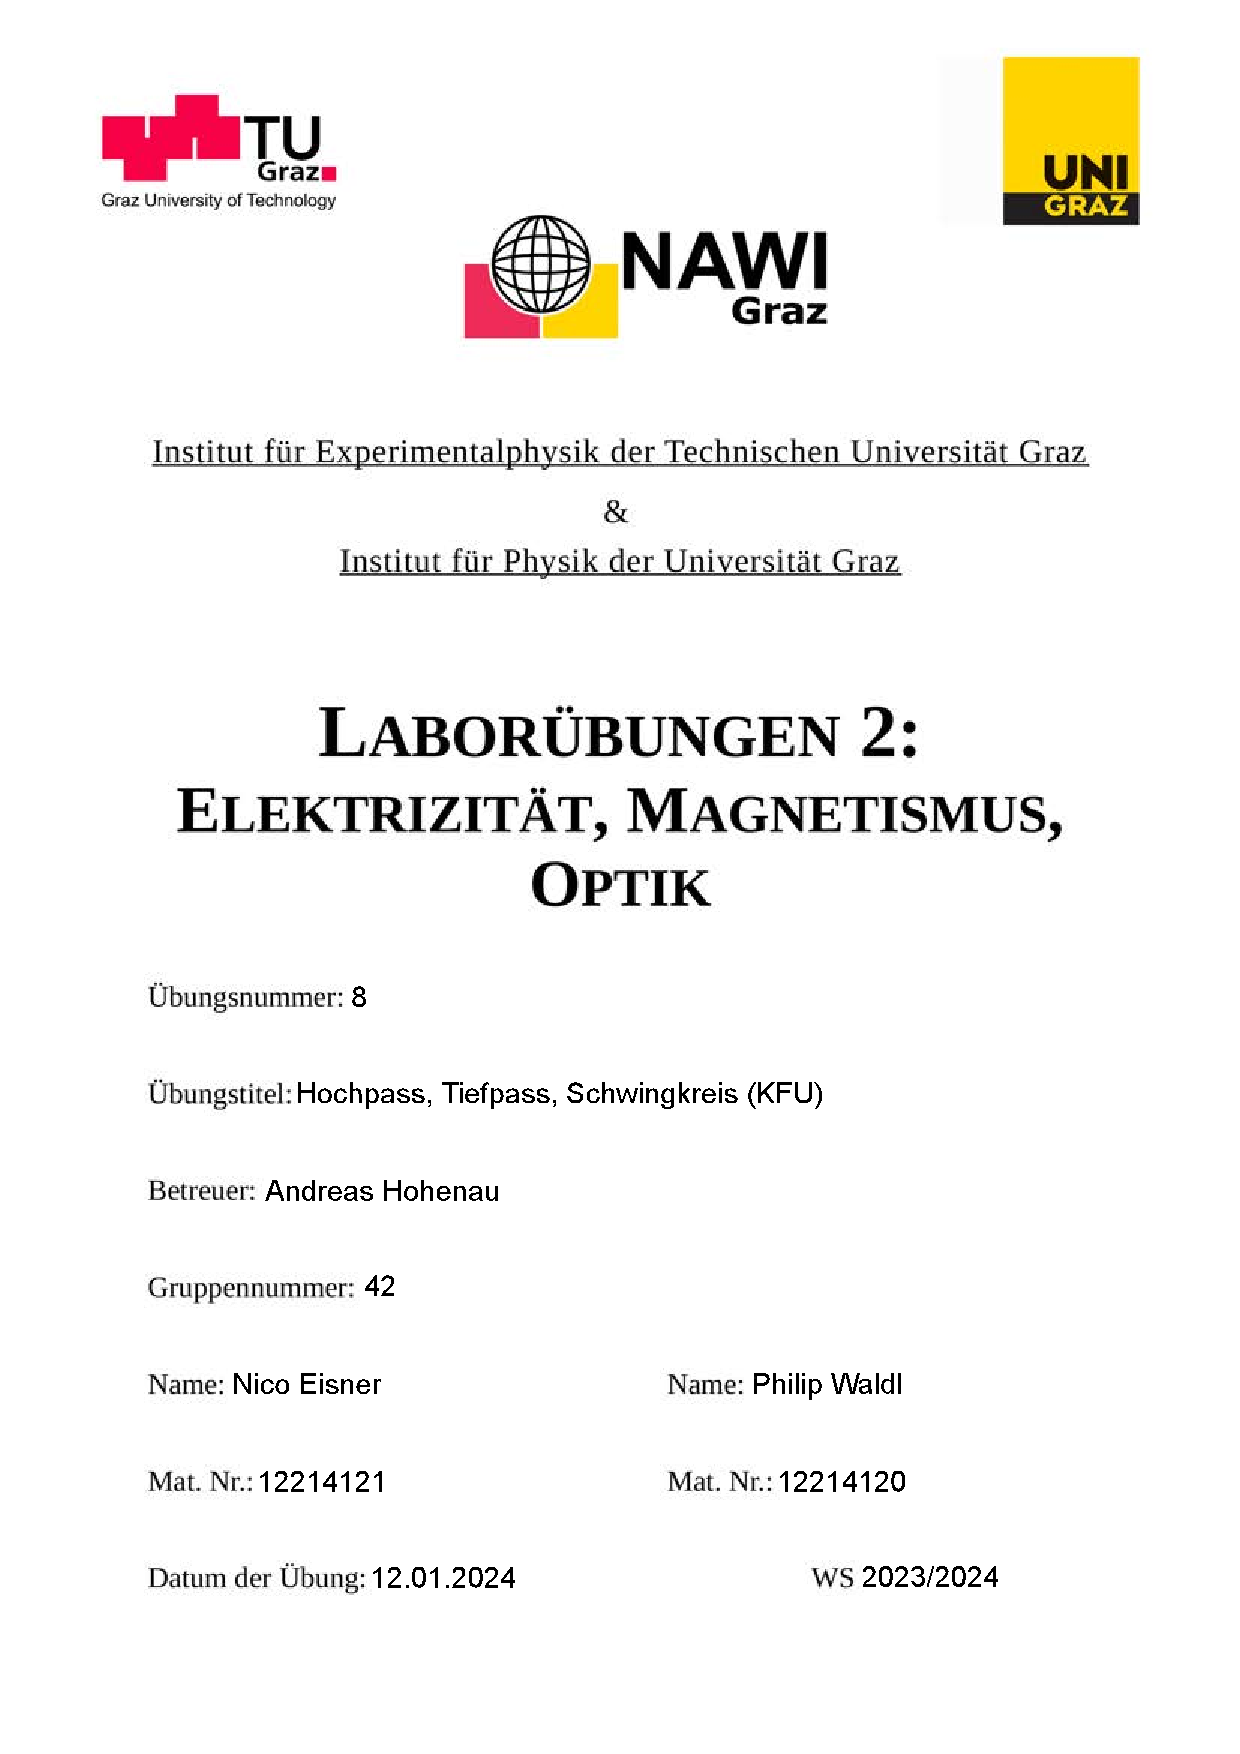
\includepdf[pages={1}]{../Deckblätter/Deckblatt_Hochpass.pdf}

\tableofcontents
\newpage

\section{Aufgabenstellung} %jo beschreibn wos gmocht host ------------------------------
Im Experiment Hochpass, Tiefpass, Schwingkreis gilt es vier Aufbaben zu erledigen. 
\\
\\
Der erste Teil besteht darin, das Bodediagramm eines CR-Hochpasses zu erstellen. 
Im zweiten Teil wird das Bodediagramm eines RC-Tiefpasses erstellt. 
Im dritten Teil wird das Schwingverhalten eines RLC Parallelschwingkreis untersucht und die Sprungantwort wird aufgenommen. 
Im vierten und letzten Teil wird das Frequenzverhalten  eines RLC Serienschwingkreises untersucht und die Resonazkurve wird aufgenommen. 
\\
\\
Alle Informationen und Methodiken wurden uns von der Technischen Universität bereitgestellt \cite{teachcenter2}. 

\section{Voraussetzungen \& Grundlagen} %Grundlagen erklären, Formeln mit erklärung
\subsection{Hochpass}
Ein Hochpass ist ein Bauteil, welches Spannungen erst ab einer gewissen Grenzfrequenz $f_G$ durch lässt. 
Ein Signal unterhalb der Grenzfrequenz $f_G$ wird nur stark gedämpft durchgelassen. 
\\
\\
Man unterscheidet unter zwei Arten eines Hochpasses, dem CR-Hochpass und dem RL-Hochpass. \\
Der CR-Hochpass besteht aus einem in Serie geschaltenen Kondensator $C$ und einem Widerstand $R$. 
Das Ausgangssignal wird am Widerstand $R$ abgegriffen. 
\\
Der RL-Hochpass besteht aus einem in Serie geschaltenen Widerstand $R$ und einer Spule $L$. Das Ausgangssignal wird an der Spule $L$ abgegriffen. 

\begin{figure}[H]
    \centering
    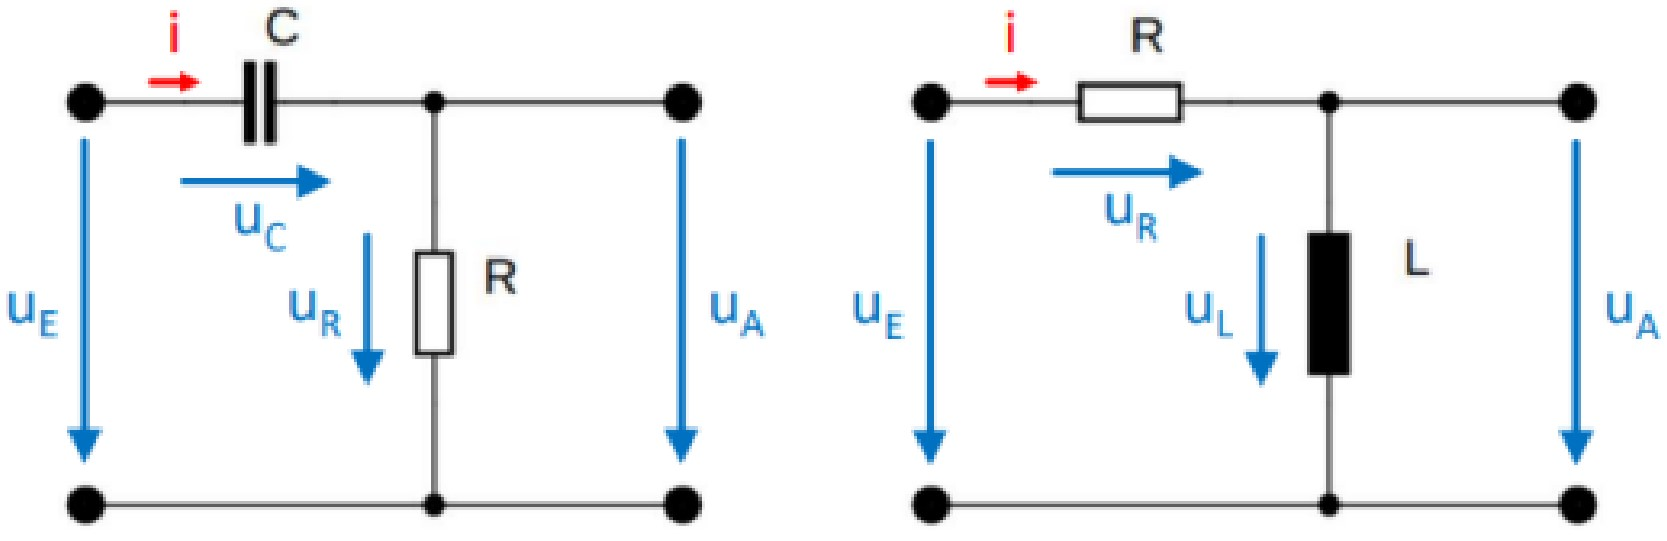
\includegraphics[width=0.6\linewidth]{nudes/HP.jpg}
    \caption{Schaltbild eines CR-Hochpass (links) und RL-Hochpass(rechts). Entnommen aus Skriptum Hochpass, Tiefpass, Schwingkreis Seite 13 \cite{teachcenter2}. }
    \label{fig:grundHochpass}
\end{figure}

\noindent
Die Grenzfrequenz $f_G$ lässt sich mit folgenden Formeln berechnen, wobei die erste für eine CR-Hochpass und die zweite für einen RL-Hochpass ist. 
\begin{equation}
    \label{eq:Grenzfrequenz CR-HP}
    \centerline{$f_G = \frac{1}{2 \pi RC}$ \\ $\Delta f_G = \vert \frac{\partial f_G}{\partial R} * \Delta R \vert + \vert \frac{\partial f_G}{\partial C} * \Delta C \vert$}
\end{equation}

\begin{equation}
    \label{eq:Grenzfrequenz RL-HP}
    \centerline{$f_G = \frac{R}{2 \pi L}$ \\ $\Delta f_G = \vert \frac{\partial f_G}{\partial R} * \Delta R \vert + \vert \frac{\partial f_G}{\partial L} * \Delta L \vert$}
\end{equation}

\noindent
Für die weiteren Berechnungen benötigt man noch den Amplituden- $\vert \underline{G}_{j \omega} \vert$ und Phasengang $\varphi$. 
Die Gleichungen für einen CR-Hochpass sehen wiefolgt aus: 

\begin{equation}
    \label{eq:Amplitudengang CR-HP}
    \centerline{$\vert \underline{G}_{j \omega} \vert = \frac{1}{\sqrt{1+\frac{1}{(\omega RC)^2}}}$ \\ $\Delta \vert \underline{G}_{j \omega} \vert = \vert \frac{\partial \vert \underline{G}_{j \omega} \vert}{\partial \omega} * \Delta \omega \vert + \vert \frac{\partial \vert \underline{G}_{j \omega} \vert}{\partial R} * \Delta R \vert + \vert \frac{\partial \vert \underline{G}_{j \omega} \vert}{\partial C} * \Delta C \vert$}
\end{equation}

\begin{equation}
    \label{eq:Phasengang CR-HP}
    \centerline{$\varphi = arctan(\frac{1}{\omega RC})$ \\ $\Delta \varphi \vert = \vert \frac{\partial \varphi}{\partial \omega} * \Delta \omega \vert + \vert \frac{\partial \varphi}{\partial R} * \Delta R \vert + \vert \frac{\partial \varphi}{\partial C} * \Delta C \vert$}
\end{equation}

\noindent
Für einen RL-Hochpass sehen die Gleichungen wiefolgt aus: 

\begin{equation}
    \label{eq:Amplitudengang RL-HP}
    \centerline{$\vert \underline{G}_{j \omega} \vert = \frac{\omega L}{\sqrt{R^2 + (\omega L)^2}}$ \\ $\Delta \vert \underline{G}_{j \omega} \vert = \vert \frac{\partial \vert \underline{G}_{j \omega} \vert}{\partial \omega} * \Delta \omega \vert + \vert \frac{\partial \vert \underline{G}_{j \omega} \vert}{\partial R} * \Delta R \vert + \vert \frac{\partial \vert \underline{G}_{j \omega} \vert}{\partial L} * \Delta L \vert$}
\end{equation}

\begin{equation}
    \label{eq:Phasengang RL-HP}
    \centerline{$\varphi = arccot( \omega \frac{L}{R})$ \\ $\Delta \varphi \vert = \vert \frac{\partial \varphi}{\partial \omega} * \Delta \omega \vert + \vert \frac{\partial \varphi}{\partial R} * \Delta R \vert + \vert \frac{\partial \varphi}{\partial L} * \Delta L \vert$}
\end{equation}

\subsection{Tiefpass}
Ein Tiefpass lässt im Gegensatz zu einem Hochpass nur Spannungen mit Frequenzen niedriger der Grenzfrequenz $f_G$ durch. 
Signale über der Grenzfrequenz werden nur stark gedämpft durchgelassen. 
\\
\\
Wie auch beim Hochpass gibt es beim Tiefpass zwei verschiedenen Arten. Der RC-Tiefpass besteht aus einem in Serie geschaltenem Widerstand $R$ und einem Kondensator $C$, wobei das Ausgangssignal am Kondensator $C$ abgegriffen wird. 
Eine weitere Realisierung ist der LR-Tiefpass, welcher aus einer Spule $L$ und einem Widerstand $R$ besteht, wo das Ausgangssignal am Widerstand abgegriffen wird. 

\begin{figure}[H]
    \centering
    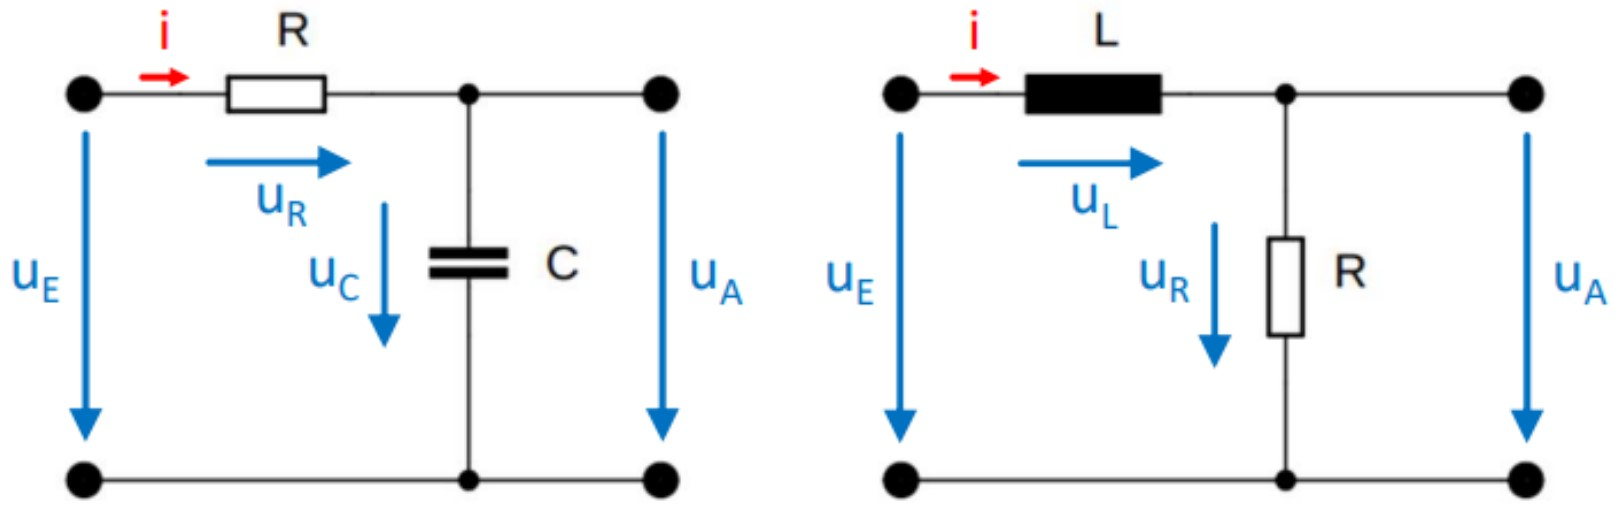
\includegraphics[width=0.6\linewidth]{nudes/TP.jpg}
    \caption{Schaltbild eines RC-Tiefpass (links) und LR-Tiefpass (rechts). Entnommen aus Skriptum Hochpass, Tiefpass, Schwingkreis Seite 13 \cite{teachcenter2}. }
    \label{fig:grundTief}
\end{figure}

\noindent
Auch bei einem Tiefpass lässt sich die Grenzfrequenz $f_G$ berechnen, wobei die Formel gleich wie bei einem Hochpass ist. Für einen RC-Tiefpass wäre das Formel \ref{eq:Grenzfrequenz CR-HP} und für einen LR-Tiefpass die Formel \ref{eq:Grenzfrequenz RL-HP}. 
\\
Für die weiteren Berechnungen benötigt man noch den Amplituden- $\vert \underline{G}_{j \omega} \vert$ und Phasengang $\varphi$. 
Der Amplitudengang $\vert \underline{G}_{j \omega} \vert$ für einen RC-Tiefpass lässt sich mit der Formel \ref{eq:Amplitudengang CR-HP} und der eines LR-Tiefpass mit der Formel \ref{eq:Amplitudengang RL-HP} berechnen. 
Der Phasengang $\varphi$ wird den folgenden Formeln berechnet, wobei die erste für einen RC-Tiefpass und die zweite für einen LR-Tiefpass ist. 

\begin{equation}
    \label{eq:Phasengang RC-TP}
    \centerline{$\varphi = -arctan( \omega RC)$ \\ $\Delta \varphi \vert = \vert \frac{\partial \varphi}{\partial \omega} * \Delta \omega \vert + \vert \frac{\partial \varphi}{\partial R} * \Delta R \vert + \vert \frac{\partial \varphi}{\partial L} * \Delta L \vert$}
\end{equation}

\begin{equation}
    \label{eq:Phasengang LR-TP}
    \centerline{$\varphi = -arctan( \omega \frac{L}{R})$ \\ $\Delta \varphi \vert = \vert \frac{\partial \varphi}{\partial \omega} * \Delta \omega \vert + \vert \frac{\partial \varphi}{\partial R} * \Delta R \vert + \vert \frac{\partial \varphi}{\partial L} * \Delta L \vert$}
\end{equation}

\subsection{RLC Parallelschwingkreis}
Dieser besteht aus der Parallelschaltung eines Kondensators $C$ und einer Spule $L$. 

\begin{figure}[H]
    \centering
    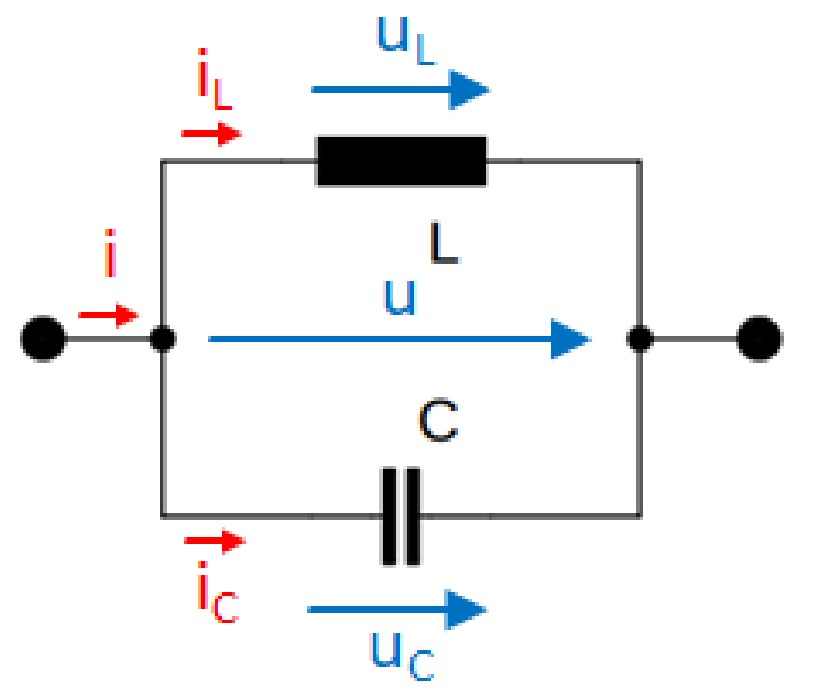
\includegraphics[width=0.6\linewidth]{nudes/RLCparallel.jpg}
    \caption{Schaltbild eines verlustfreien RLC Parallelschwingkreises. Entnommen aus Skriptum Hochpass, Tiefpass, Schwingkreis Seite 19 \cite{teachcenter2}. }
    \label{fig:grundParallel}
\end{figure}

\noindent
Der Parallelschwingkreis funktioniert wiefolgt. Der Kondensator wird durch eine Energiequelle aufgeladen und erzeugt dabei ein elektrisches Feld. 
Klemmt man die Energiequelle ab, so entlädt sich der Kondenstor und baut in der Spule ein Magnetisches Feld auf, welches die Feldenergie des Kondensators übernimmt. Fließt kein Strom mehr, so wirkt die Spule dem Entgegen und versucht diesen Aufrecht zu erhalten. 
Die Spule baut ihr Magnetfeld ab und lädt den Kondensator wieder auf, jedoch mit einem umgekehrten Vorzeichen. Ist die Energie des Magnetfeldes abgebaut, so ist die gesamte Energie wieder als elektrische Energie beim Kondensator und der vorgang wiederholt sich. 
\\
Dies ist jedoch nur bei ungedämpften Schwingkreisen der Fall, bei realen Schwingkreisen sind die Verluste des Kondensators und der Spule zu berücksichtigen. 
\\
\\
Die Eigenfrequenz $\omega_0$ lässt sich mit der Thomsonschen Schwingungsgleichung berechnen. 

\begin{equation}
    \label{eq:Eigenfrequenz}
    \centerline{$\omega_0 = \sqrt{\frac{1}{LC}}$ \\ $\Delta \omega_0 = \vert \frac{\partial \omega_0}{\partial L} * \Delta L \vert + \vert \frac{\partial \omega_0}{\partial C} * \Delta C \vert$}
\end{equation}

\noindent
Mithilfe der Eigenfrequenz $\omega_0$ lässt sich die Frequenz $f_0$ bestimmen. 

\begin{equation}
    \label{eq:Frequenz}
    \centerline{$f_0 = \frac{\omega_0}{2 \pi}$}
\end{equation}

\noindent
Die Güte $Q$ entspricht jener des Serienschwingkreises als Kehrwert. 

\subsection{RLC Serienschwingkreis}
Im Gegensatz zu dem RLC Parallelschwingkreis besteht der Serienschwingkreis aus einem Kondensator $C$ welcher in Serie mit einer Spule $L$ geschalten ist. 
Die elektromagnetische Energie schwingt zwischen den Bauteilen. Im Kondensator wird sie als elektrische Energie und in der Spule als magnetische Energie gespeichert. 
Ideal kann die Energie zwischen den Bauteilen ewig hin und her pendeln. 
In der Realität treten Verluste auf, welche als Widerstand $R$ beschrieben werden. 

\begin{figure}[H]
    \centering
    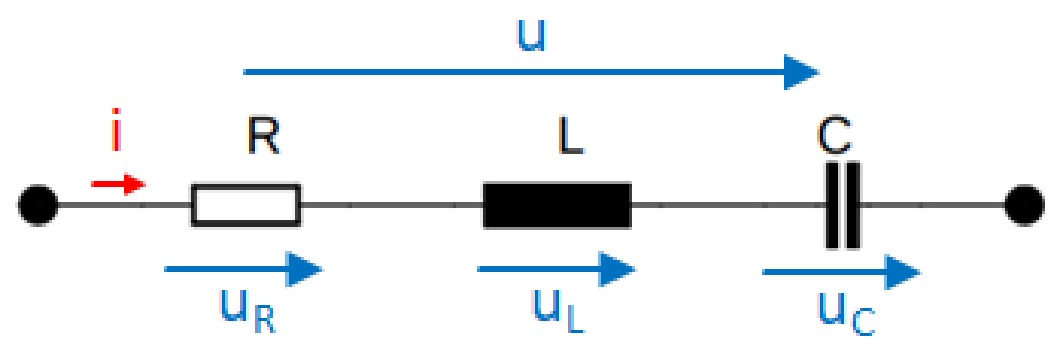
\includegraphics[width=0.6\linewidth]{nudes/RLCseriell.jpg}
    \caption{Schaltbild eines RLC Seriellschwingkreises. Entnommen aus Skriptum Hochpass, Tiefpass, Schwingkreis Seite 24 \cite{teachcenter2}. }
    \label{fig:grundSeriell}
\end{figure}

\noindent
Um die Obere- und Untere Grenzfrequenz zu bestimmen $\omega_{go}$ \& $\omega_{gu}$ benötigt man die Grenzfrequenz $\omega_0$ sowie den Widerstand $R$ und die Spule $L$. 

\begin{equation}
    \label{eq:wgo}
    \centerline{$\omega_{go} = \sqrt{\omega_0^2 + (\frac{R}{2L})^2} + (\frac{R}{2L})$ \\ $\Delta \omega_{go}= \vert \frac{\partial \omega_{go}}{\partial \omega_0} * \Delta \omega_0 \vert + \vert \frac{\partial \omega_{go}}{\partial L} * \Delta L \vert + \vert \frac{\partial \omega_{go}}{\partial R} * \Delta R \vert$}
\end{equation}

\begin{equation}
    \label{eq:wgu}
    \centerline{$\omega_{gu} = \sqrt{\omega_0^2 + (\frac{R}{2L})^2} - (\frac{R}{2L})$ \\ $\Delta \omega_{go}= \vert \frac{\partial \omega_{go}}{\partial \omega_0} * \Delta \omega_0 \vert + \vert \frac{\partial \omega_{go}}{\partial L} * \Delta L \vert + \vert \frac{\partial \omega_{go}}{\partial R} * \Delta R \vert$}
\end{equation}

\noindent
Aus diesen lässt sich die Bandbreite $B$ bestimmen. 

\begin{equation}
    \label{eq:Bandbreite}
    \centerline{$B = \omega_{go} - \omega_{gu}$}
\end{equation}

\noindent
Die Güte $Q$ eines Schwingkreises ist hauptsächlich durch die der Spule $L$ bestimmt. Sie lässt sich aber auch durch den Kehrwert der Dämpfung $d$ bestimmen. 

\begin{equation}
    \label{eq:Güte}
    \centerline{$Q = \frac{1}{d} = \frac{\omega_0}{B}$ \\ $\Delta Q = \vert \frac{\partial Q}{\partial \omega_0} * \Delta \omega_0 \vert + \vert \frac{\partial Q}{\partial B} * \Delta B \vert$}
\end{equation}


\section{Versuchsanordnung} %mit skizze kurz beschreiben ------------------------------
Die Bilder der Schaltpläne wurden dem Skript Hochpass, Tiefpass, Schwingkreis entnommen \cite{teachcenter2}. 
\\
\\
Der Aufbau der einzelnen Schaltungen erfolgt auf einem Steckbrett mit BNC- und 4mm Buchsen. 
\\
Die verwendeten Komponenten werden in Kapitel Versuchsdurchführung beschrieben. 

\begin{figure}[H]
    \centering
    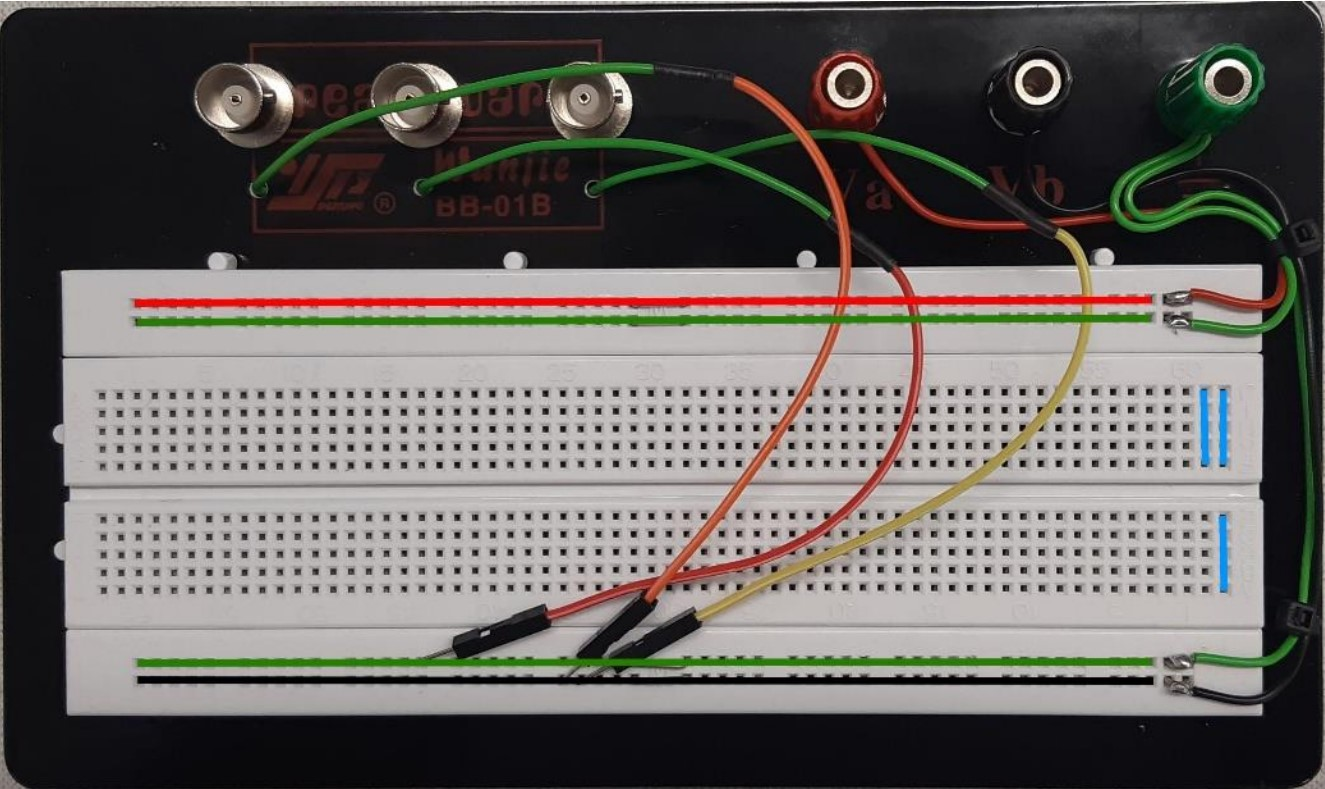
\includegraphics[width=0.6\linewidth]{nudes/steckbrett.jpg}
    \caption{Steckbrett mit BNC und 4mm Buchsen. Entnommen aus Skriptum Hochpass, Tiefpass, Schwingkreis Seite 2 \cite{teachcenter2}.}
    \label{fig:steckbrett} 
\end{figure}

\subsection{Hochpass}

\begin{figure}[H]
    \begin{minipage}[b]{.5\linewidth} % [b] => Ausrichtung an \caption
        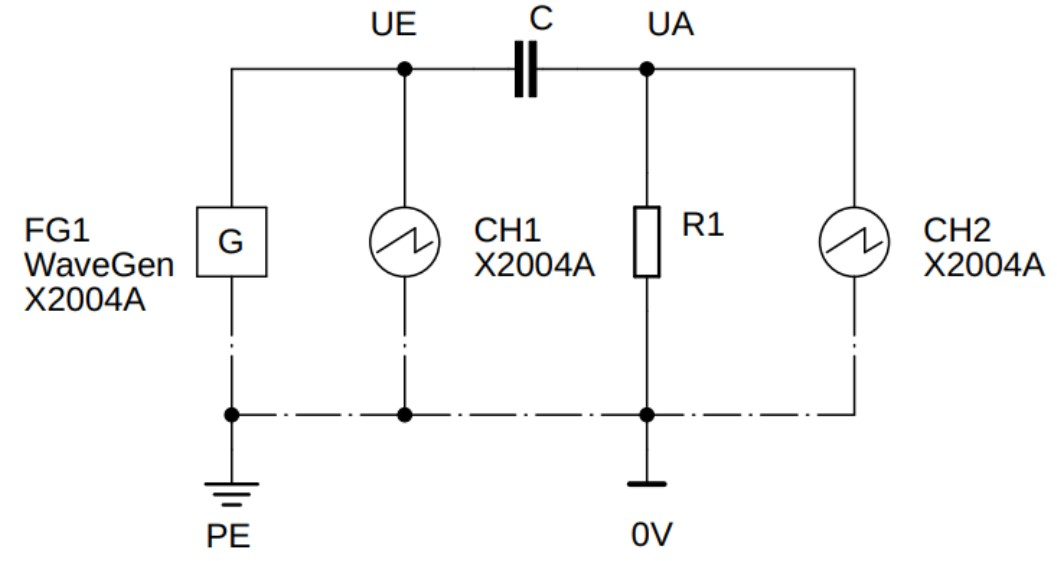
\includegraphics[width=1\linewidth]{nudes/Aufgabe 1 schaltplan.jpg}
        \caption{Schaltplan }
        \label{fig:a1s}
    \end{minipage}
    \hspace{0.01\linewidth}% Abstand zwischen Bilder
    \begin{minipage}[b]{.5\linewidth} % [b] => Ausrichtung an \caption
        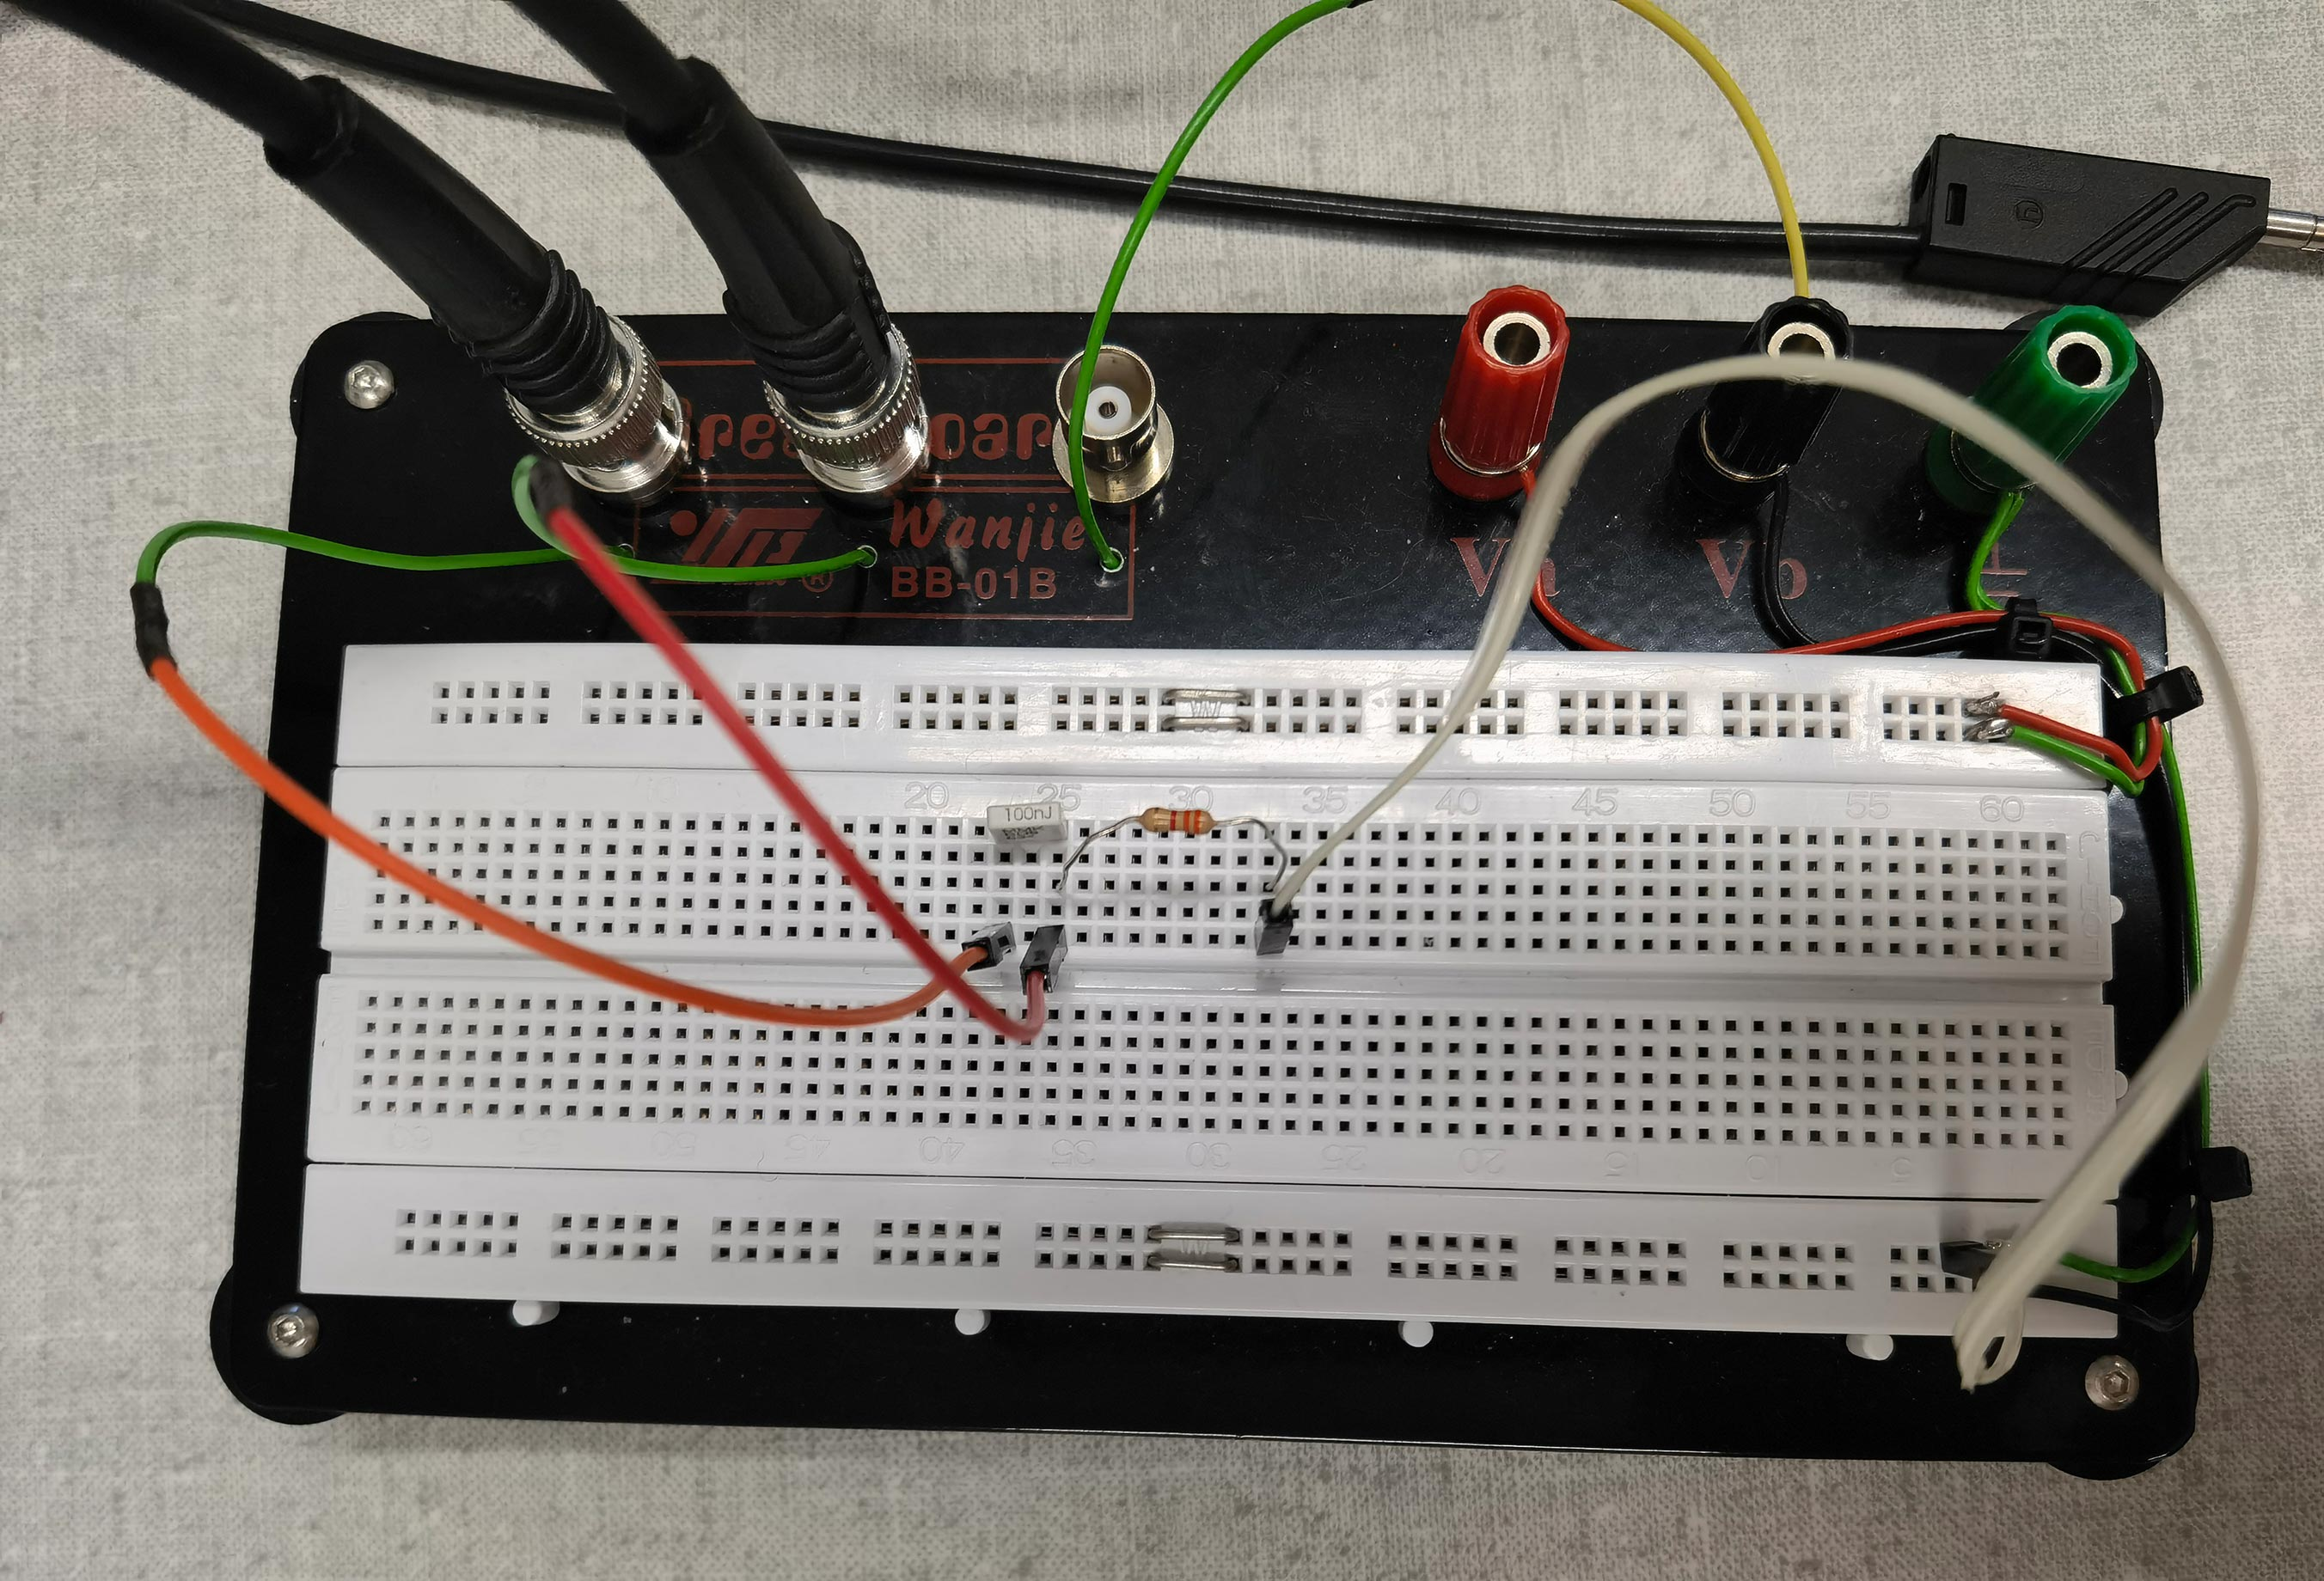
\includegraphics[width=1\linewidth]{nudes/a1 brett.jpg}
    \caption{Steckbrett}
    \label{fig:a1b}
    \end{minipage}
\end{figure}


\subsection{Tiefpass}

\begin{figure}[H]
    \begin{minipage}[b]{.5\linewidth} % [b] => Ausrichtung an \caption
        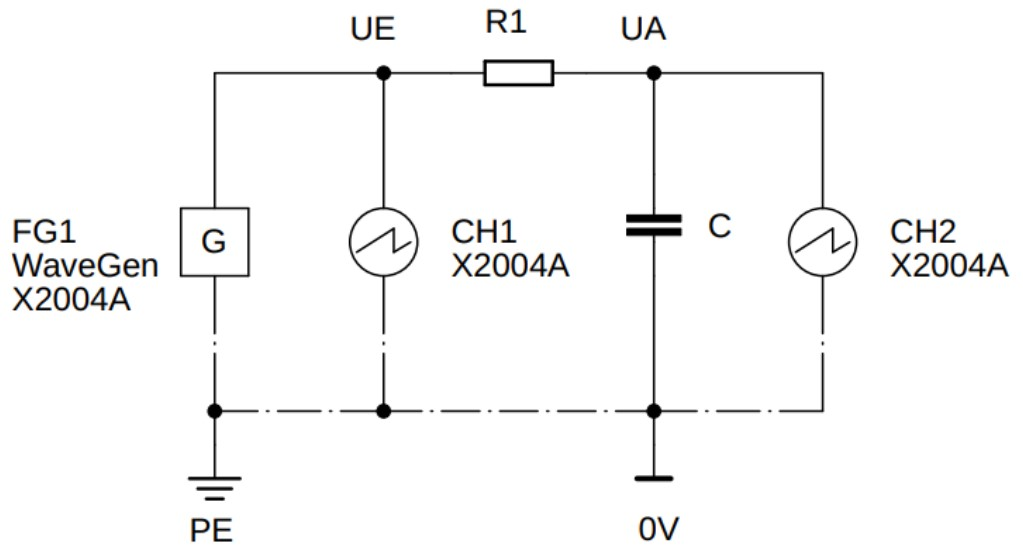
\includegraphics[width=1\linewidth]{nudes/Aufgabe 2 schaltplan.jpg}
        \caption{Schaltplan }
        \label{fig:a2s}
    \end{minipage}
    \hspace{0.01\linewidth}% Abstand zwischen Bilder
    \begin{minipage}[b]{.5\linewidth} % [b] => Ausrichtung an \caption
        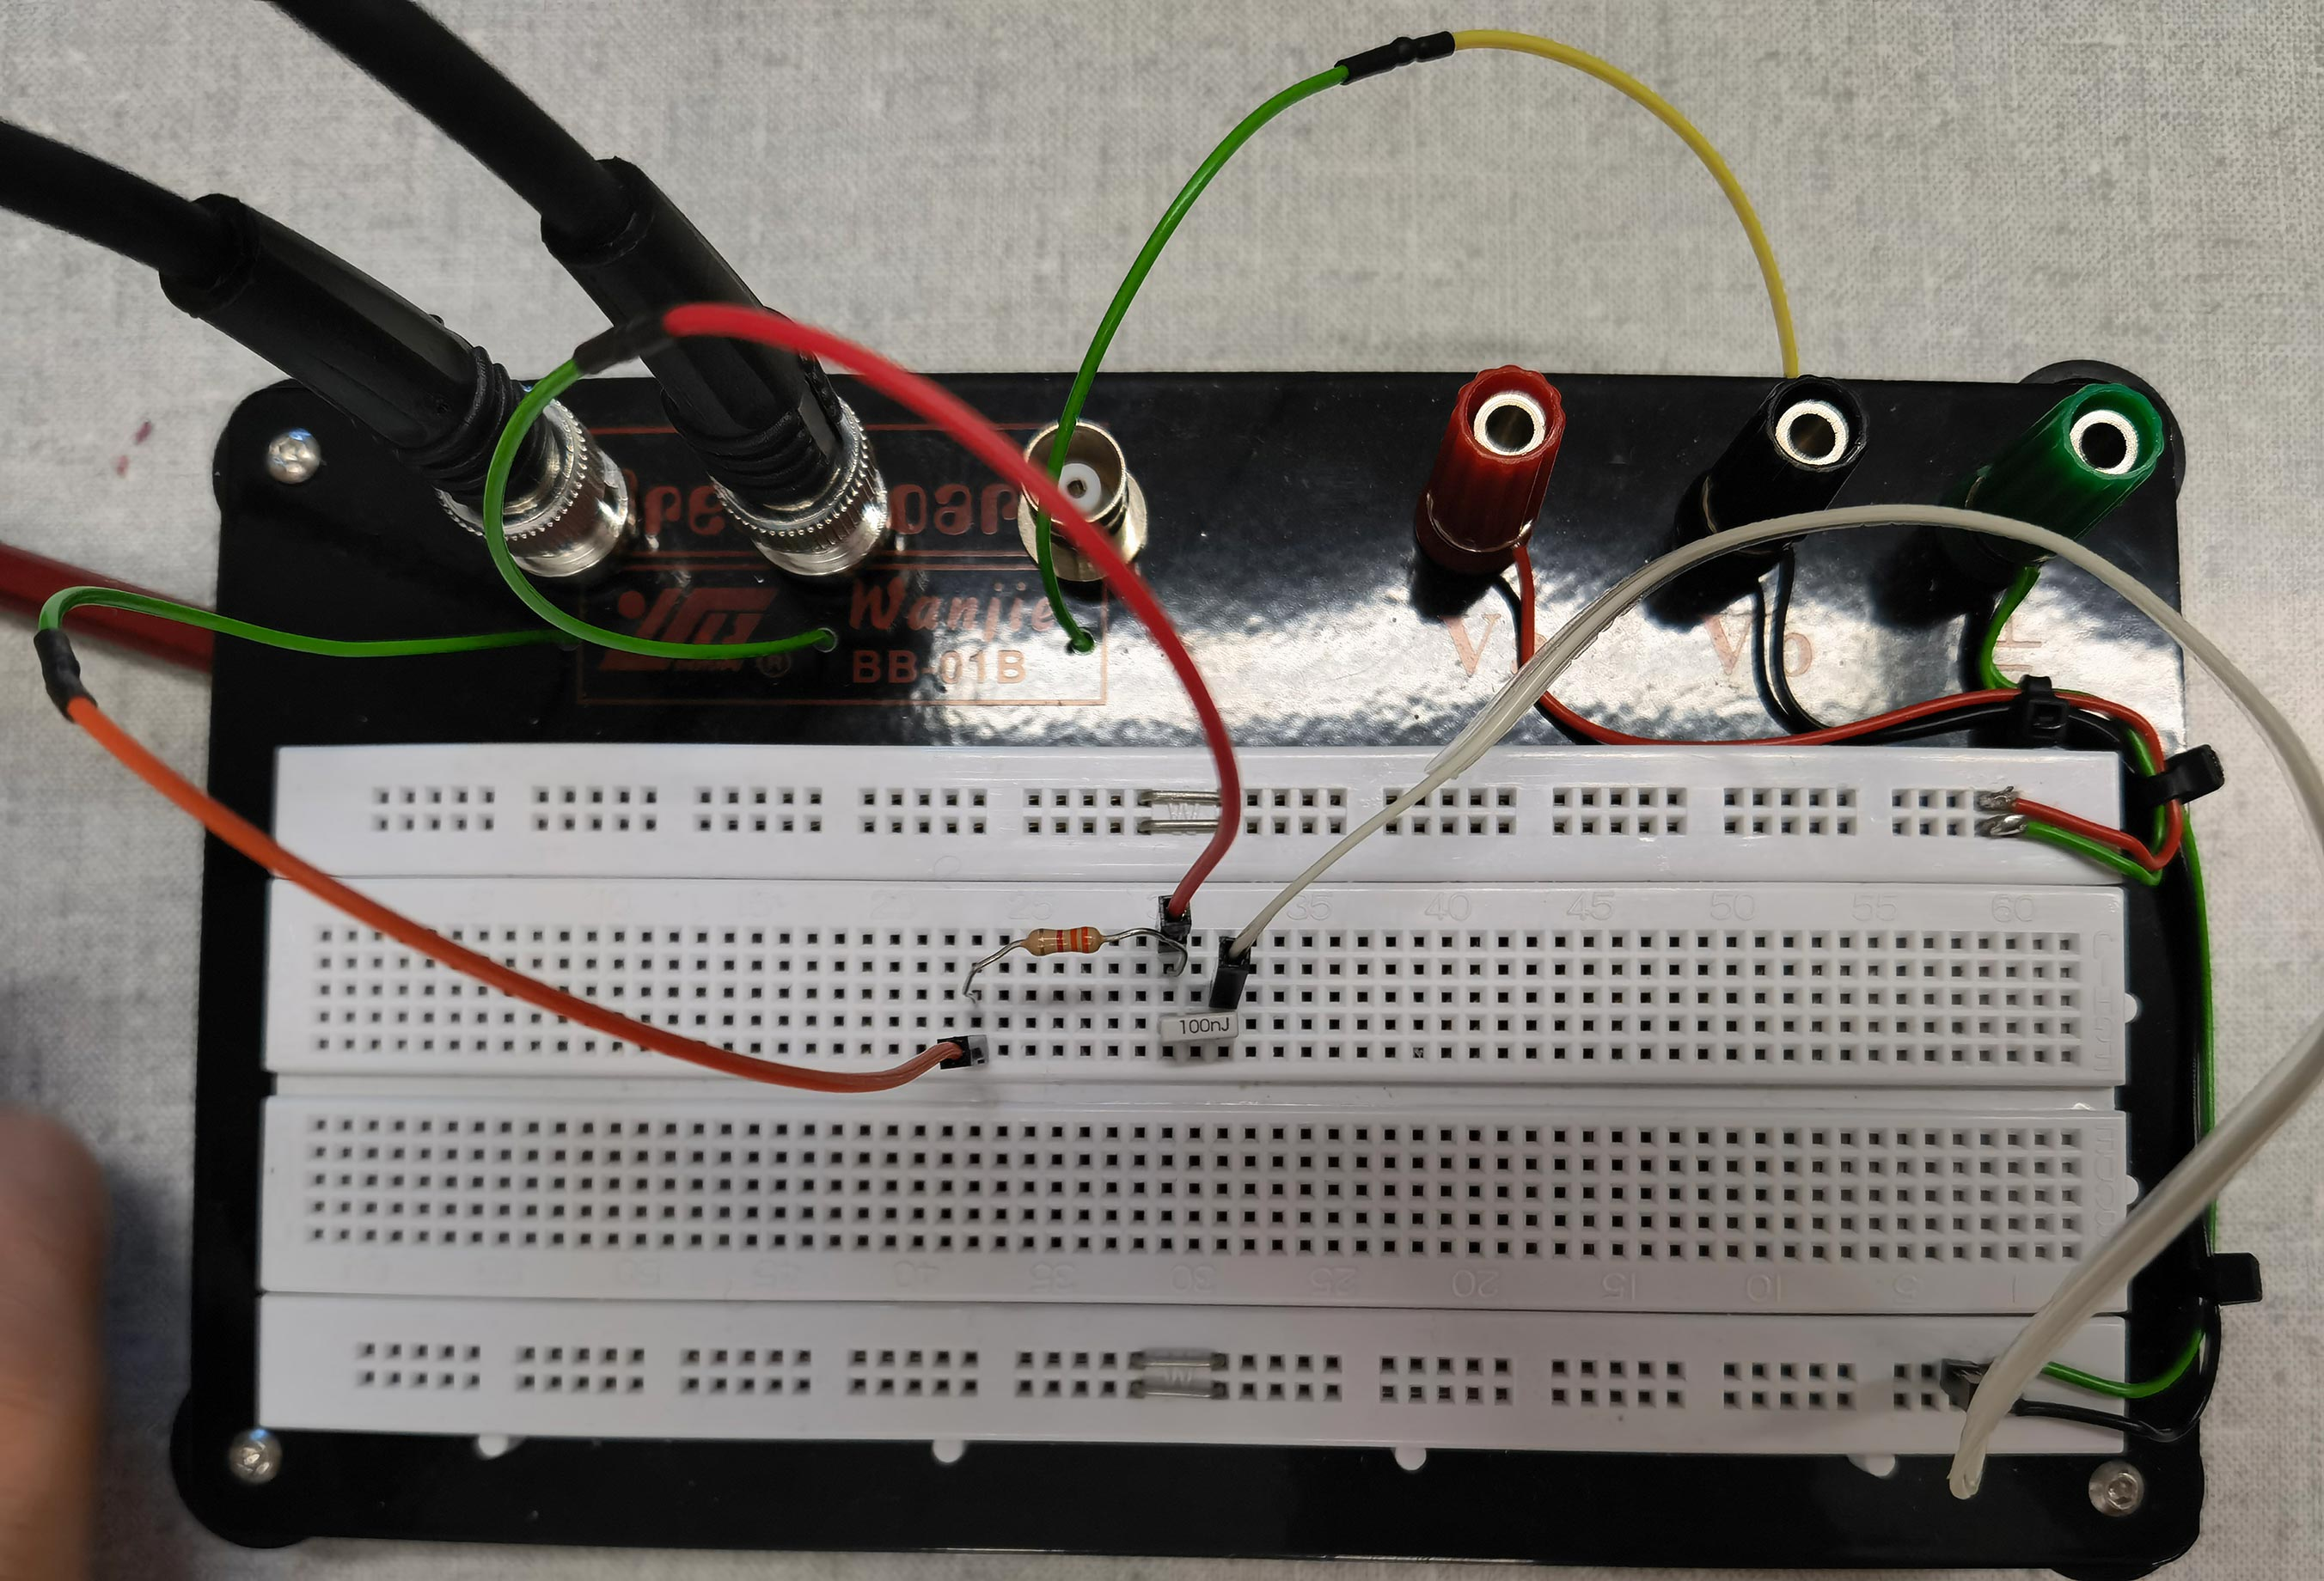
\includegraphics[width=1\linewidth]{nudes/a2 brett.jpg}
    \caption{Steckbrett}
    \label{fig:a2b}
    \end{minipage}
\end{figure}


\subsection{RLC Parallelschwingkreis}

\begin{figure}[H]
    \begin{minipage}[b]{.5\linewidth} % [b] => Ausrichtung an \caption
        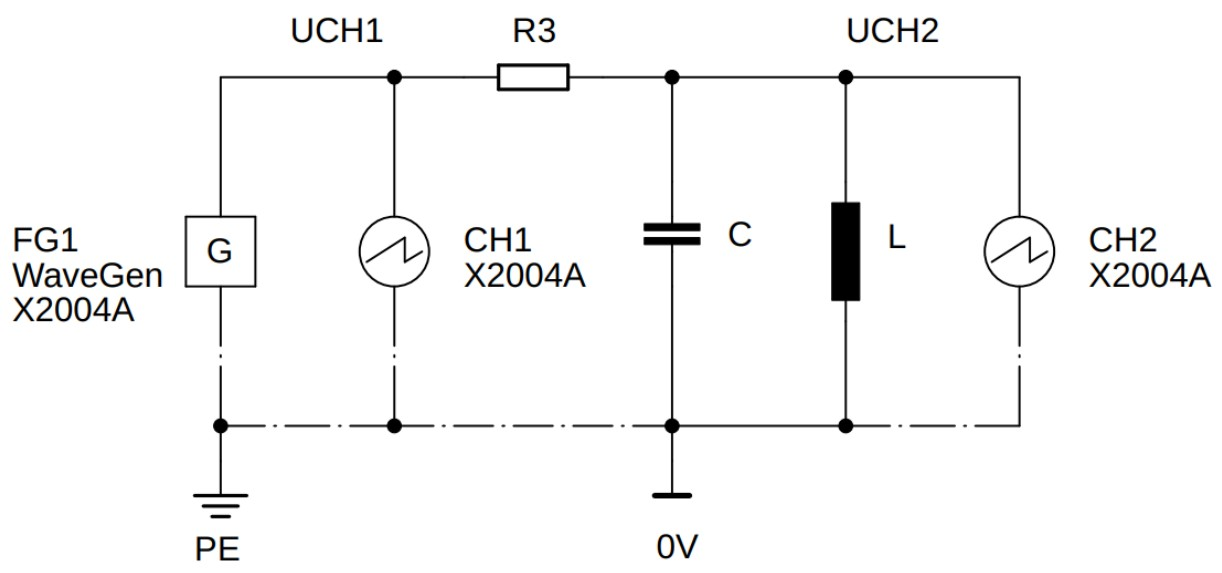
\includegraphics[width=1\linewidth]{nudes/Aufgabe 3 schaltplan.jpg}
        \caption{Schaltplan }
        \label{fig:a3s}
    \end{minipage}
    \hspace{0.01\linewidth}% Abstand zwischen Bilder
    \begin{minipage}[b]{.5\linewidth} % [b] => Ausrichtung an \caption
        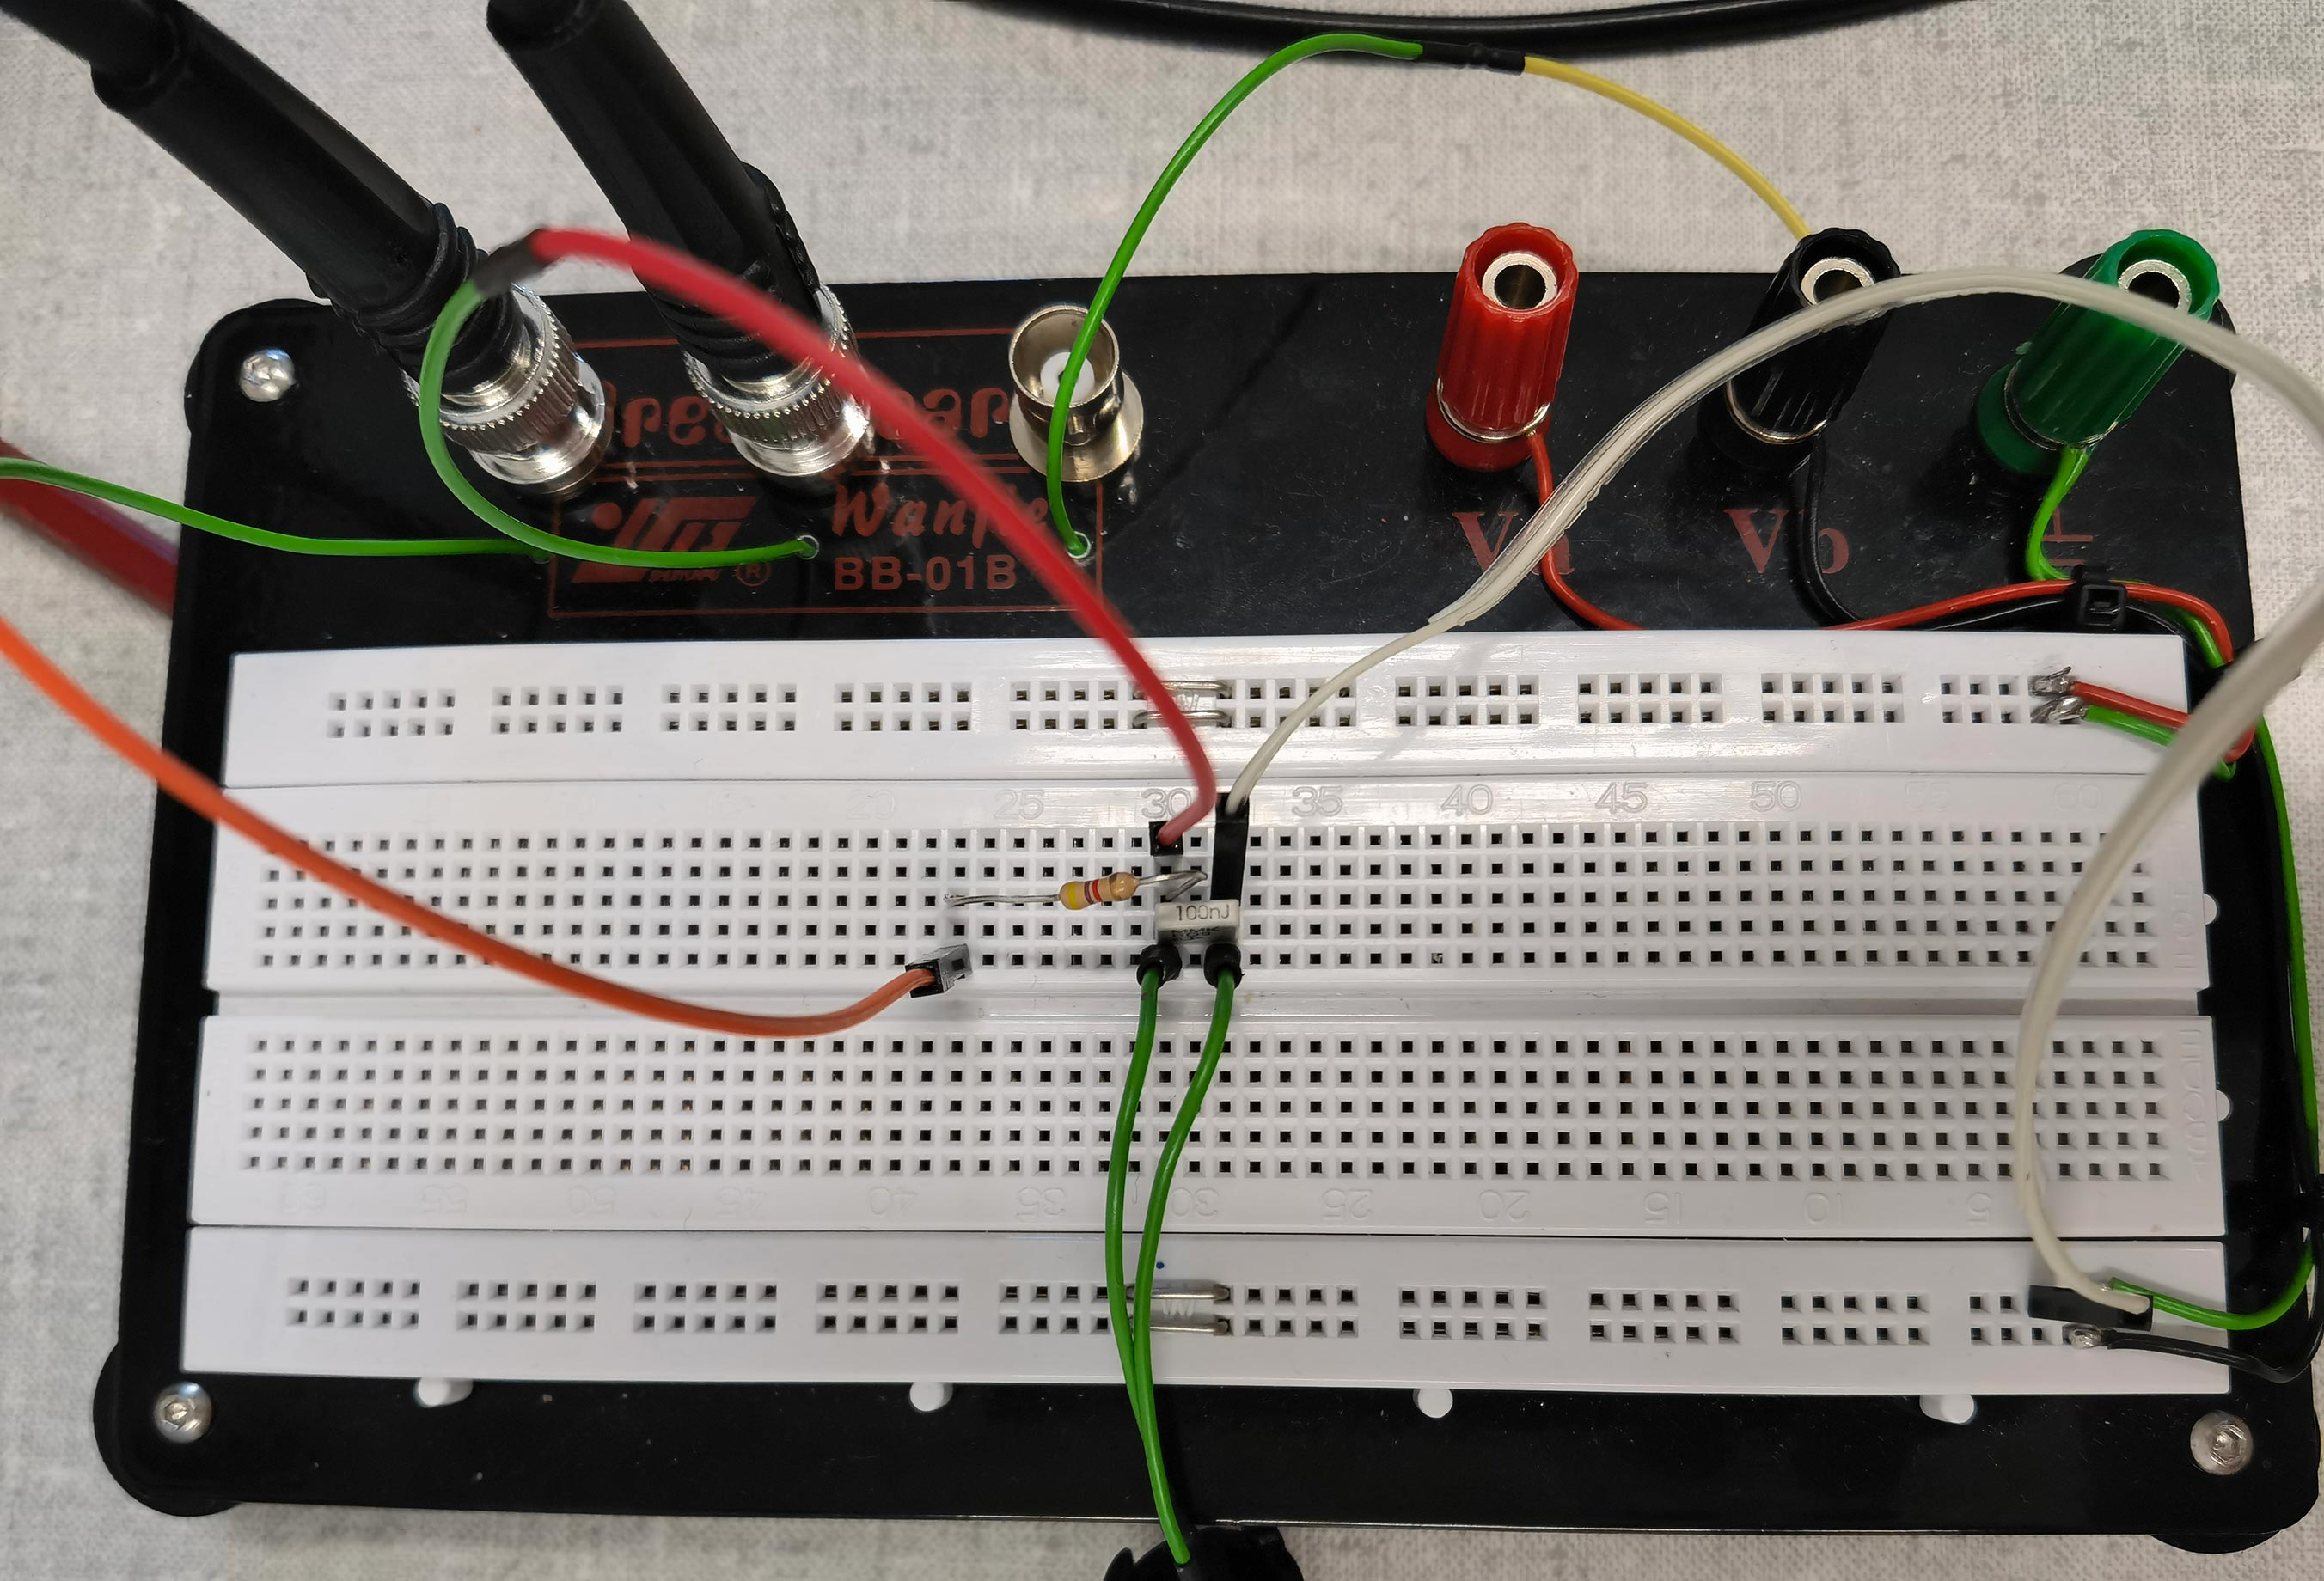
\includegraphics[width=1\linewidth]{nudes/a3 brett.jpg}
    \caption{Steckbrett}
    \label{fig:a3b}
    \end{minipage}
\end{figure}


\subsection{RLC Seriellschwingkreis}

\begin{figure}[H]
    \begin{minipage}[b]{.5\linewidth} % [b] => Ausrichtung an \caption
        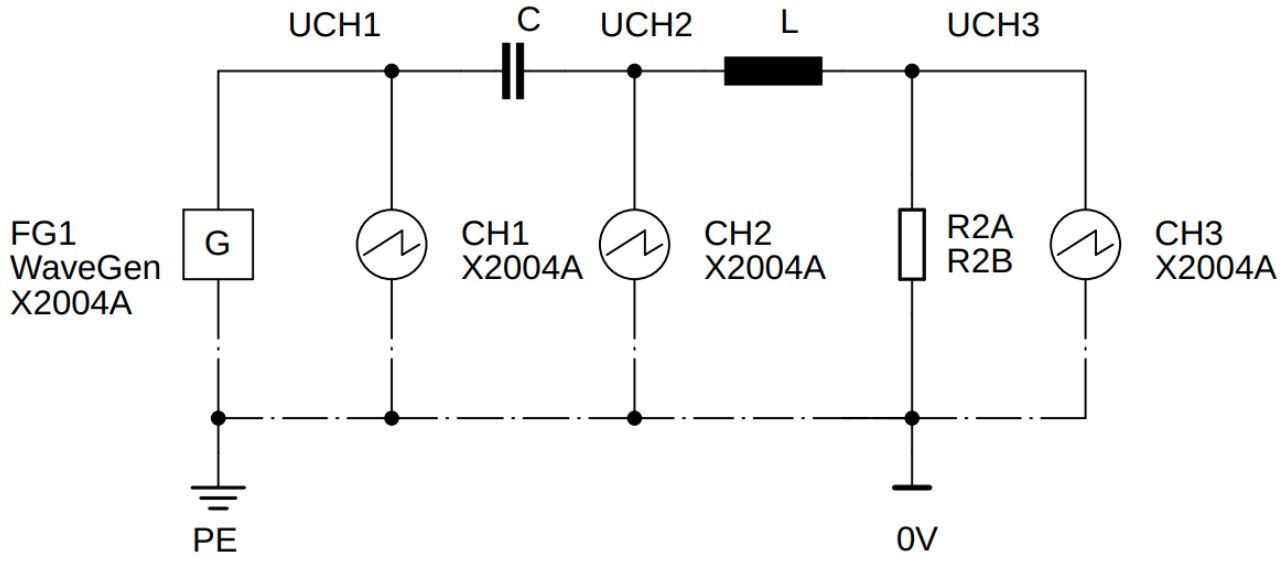
\includegraphics[width=1\linewidth]{nudes/Aufgabe 4 schaltplan.jpg}
        \caption{Schaltplan }
        \label{fig:a4s}
    \end{minipage}
    \hspace{0.01\linewidth}% Abstand zwischen Bilder
    \begin{minipage}[b]{.5\linewidth} % [b] => Ausrichtung an \caption
        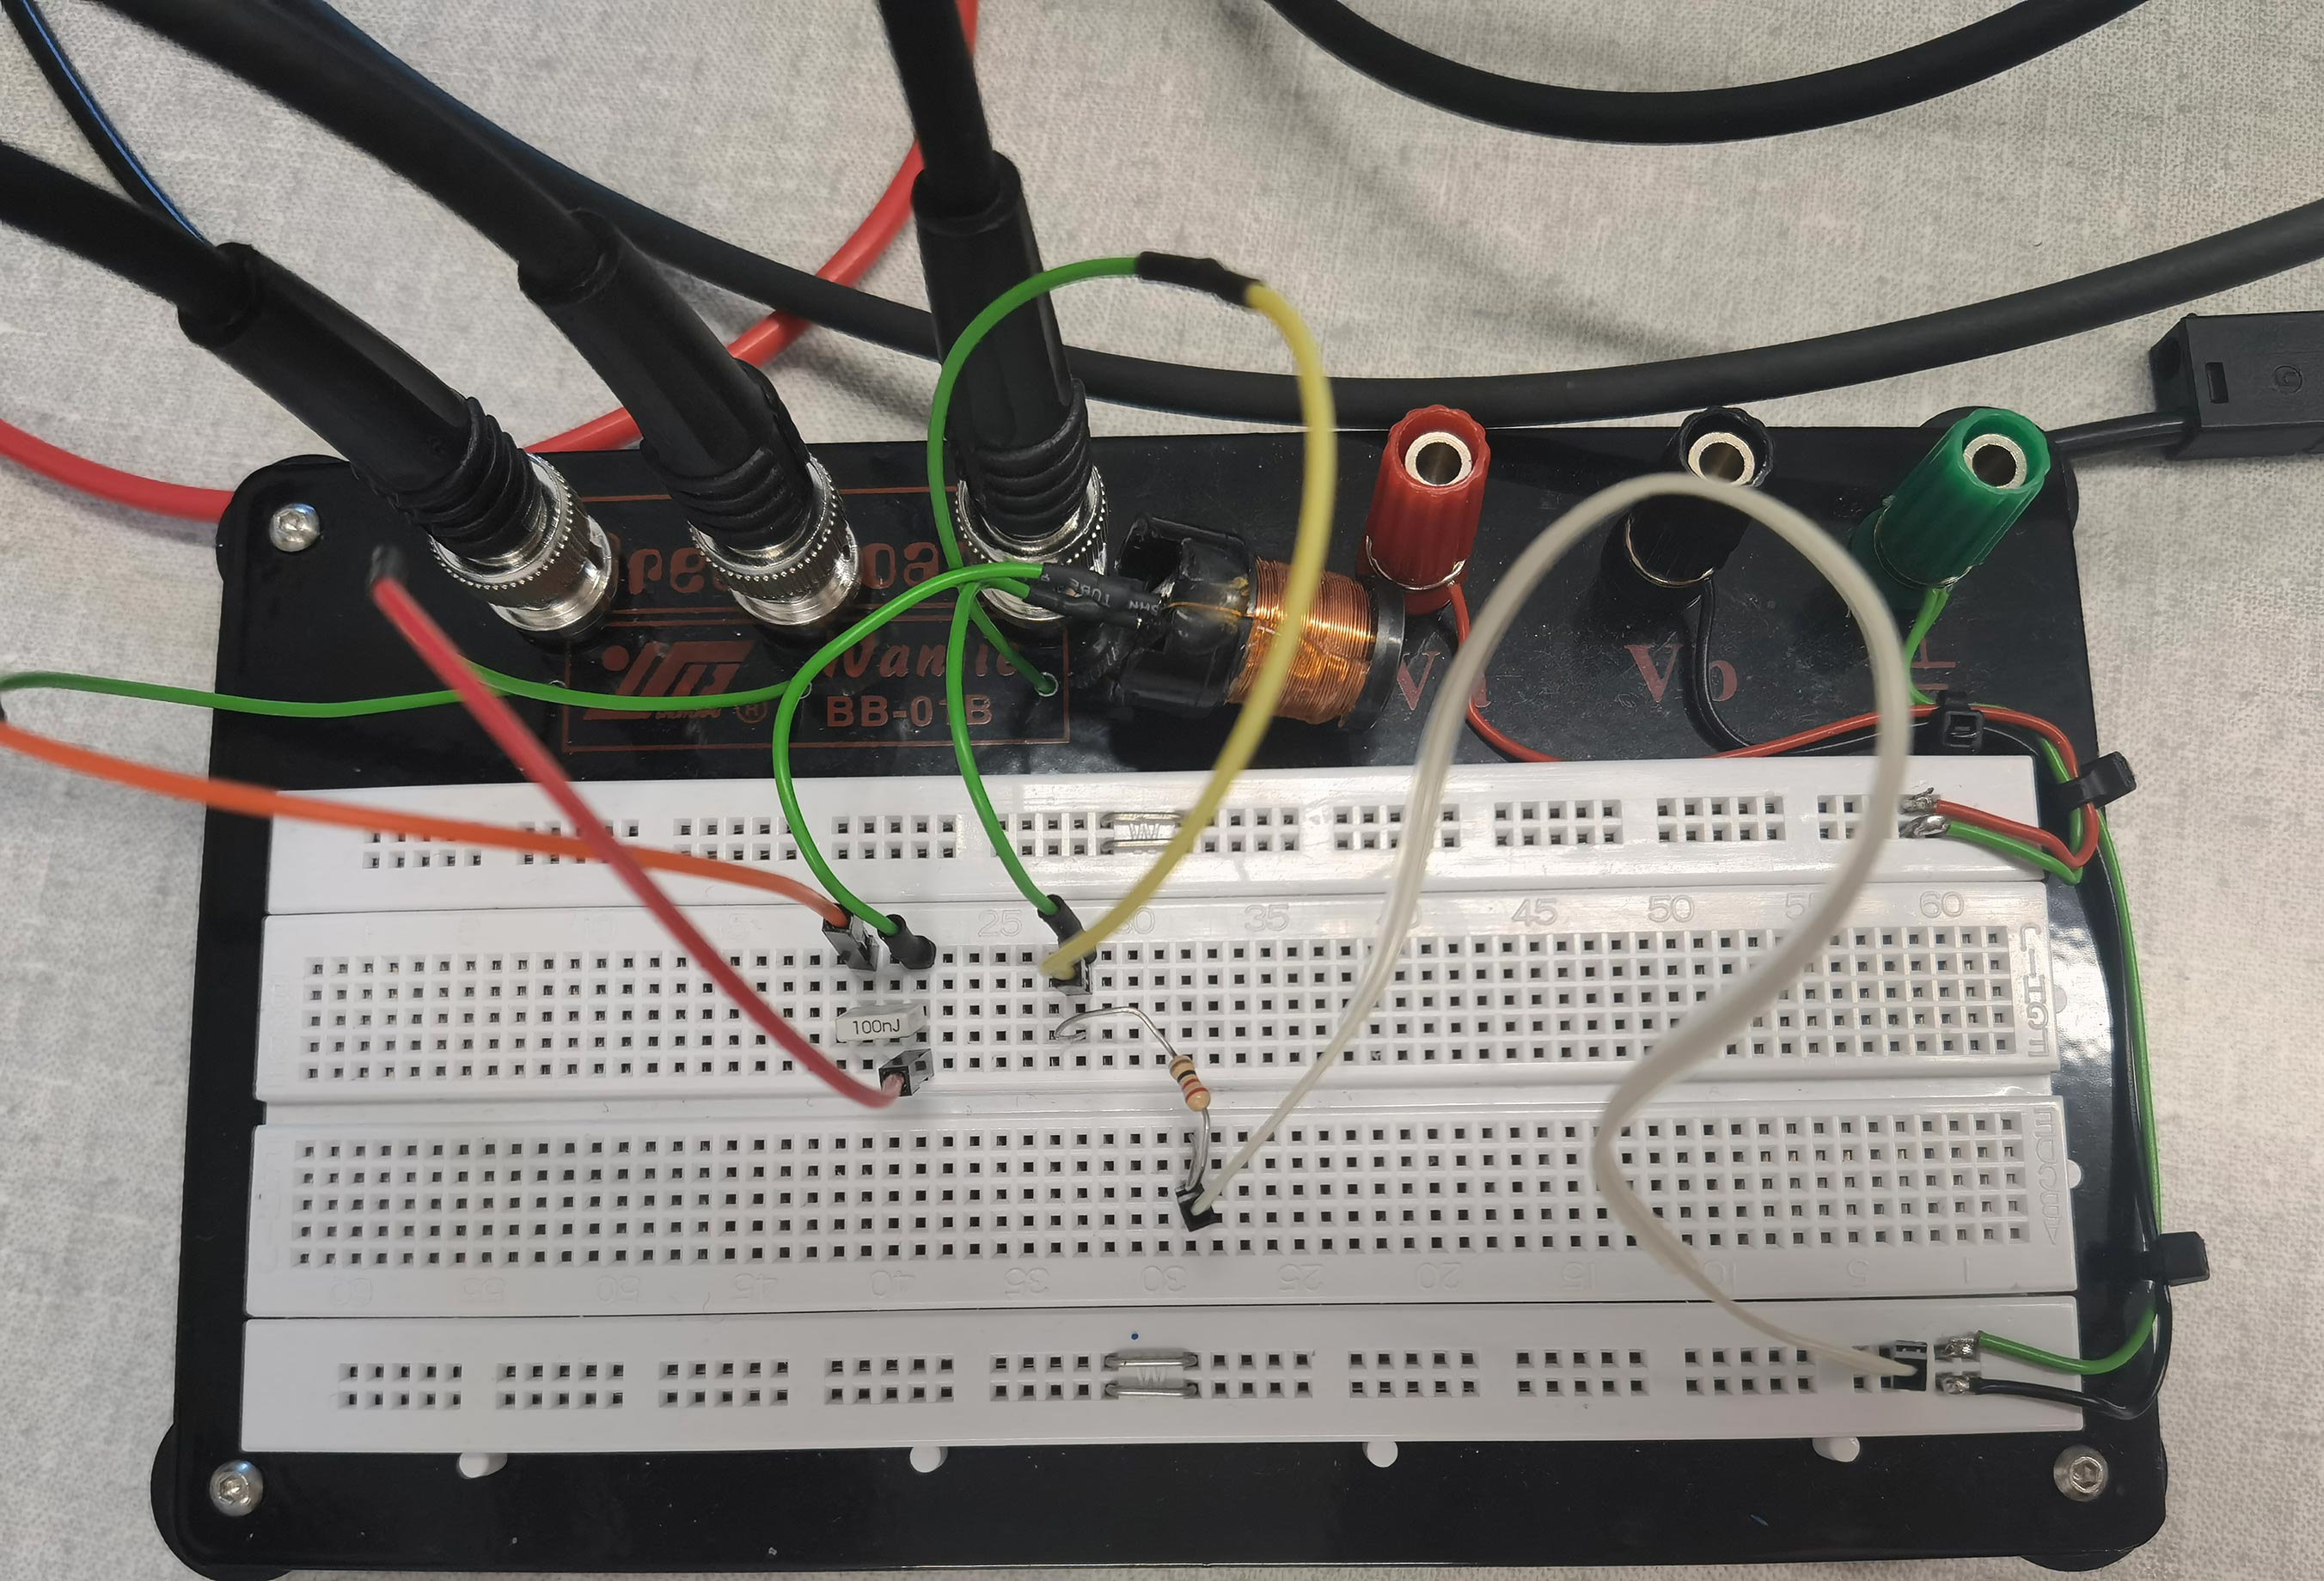
\includegraphics[width=1\linewidth]{nudes/a4 brett.jpg}
    \caption{Steckbrett}
    \label{fig:a4b}
    \end{minipage}
\end{figure}


\section{Geräteliste} %jo holt a listn ------------------------------
Unsicherheiten des Kondensators und der Spule implizit angenommen. 
    \begin{table}[H]
        \centering
        \caption{Im Versuch verwendete Geräte und Utensilien.}
        \label{tab:geraete}
        \begin{tabular}{| l | l | l |}
            \hline
            Gerät    & Gerätenummer  & Unsicherheit \\
            \hline
            Oszilloskop             & Keysight DSOX2004A        & {n.a} \\
            Funktionsgenerator Oszi & Keysight DSOX2004A        & {n.a} \\
            Multimeter              & Fluke 175                 & $\pm (0.9 + 1 dig.)$ \cite{fluke} \\
            Steckbrett              & {n.a}                     & {n.a} \\
            Widerstände             & R1 = 3282 $\Omega$        & $\pm 30 \Omega$ \\
                                    & R2A = 22 $\Omega$         & $\pm 1 \Omega$ \\
                                    & R3 = 4696 $\Omega$        & $\pm 42 \Omega$ \\
            Kondensator             & C = 100nF                 & $\pm 1 nF$ \\
            Spule                   & L = 10mH                  & $\pm 10 \mu H$ \\
            \hline
        \end{tabular}
    \end{table}


\section{Versuchsdurchführung \& Messergebnisse} %nachvollziehbar und klar dargestellt ------------------------------
\subsection{Hochpass}
Der Versuch wird wie in Abbildung \ref{fig:a1b} aufgebaut. 
Der Widerstand $R1$ wird mithilfe des Multimeters bestimmt und beträgt $R1 = (3282 \pm 30)\Omega $. 
Um die richtige Frequenz $f$ am Funktionsgenerator des Oszilloskopes einzustellen benötigt man die Grenzfrequenz $f_g$, welche mit der Formel \ref{eq:Grenzfrequenz CR-HP} bestimmt wird. 
Anschließend nimmt man 20 Werte auf. Es ist dabei zu beachten Werte oberhalb und unterhalb der Grenzfrequenz $f_g = (485 \pm 10)Hz $ aufzunehmen. 
Am Oszilloskop liest man den Spitze-Spitze Wert ($U_{pp}$)der jeweiligen Channels ab, sowie den Phasenversatz $\varphi_{EA}$. Wobei $U_{CH1} = U_E$ und $U_{CH2} = U_A$. 
Diese Werte lassen sich über die ''Measure'' Funktion des Oszilloskopes anzeigen. 

\begin{table}[H]
    \centering
    \caption{Messwerte der Eingangsspannung $U_E$ und Ausgangsspannung $U_A$ sowie Signalfrequenz $f$ und Phasenwinkel $\varphi_{EA}$. }
    \label{tab:mess1}
    \begin{tabular}{| l | l | l | l |}
        \hline
        $f$ $\pm$ 0.5 / Hz   & $U_E$ $\pm$ 0.01 / V   & $U_A$ $\pm$ 0.01 / V  & $\varphi_{EA}$ $\pm$ 1 / deg. \\
        \hline
        10    & 2.05 & 0.08  & -88 \\
        50    & 2.05 & 0.24  & -83 \\
        100   & 2.05 & 0.44  & -77 \\
        150   & 2.05 & 0.64  & -72 \\
        200   & 2.05 & 0.80  & -66 \\
        250   & 2.05 & 0.96  & -61 \\
        300   & 2.05 & 1.11  & -57 \\
        350   & 2.05 & 1.21  & -53 \\
        400   & 2.05 & 1.33  & -49 \\
        \textbf{480} & \textbf{2.03} & \textbf{1.45}  & \textbf{-44} \\
        600   & 2.01 & 1.61  & -39 \\
        1000  & 2.01 & 1.81  & -26 \\
        1500  & 2.01 & 1.93  & -17 \\
        2000  & 2.01 & 1.97  & -13 \\
        2500  & 2.01 & 1.97  & -10 \\
        3000  & 2.01 & 1.99  & -8  \\
        3500  & 2.01 & 1.99  & -7  \\
        4000  & 2.01 & 2.01  & -6  \\
        6000  & 2.01 & 2.01  & -4  \\
        10000 & 2.01 & 2.01  & -2  \\
        \hline
    \end{tabular}
\end{table}

\subsection{Tiefpass}
Der Versuch wird wie in Abbildung \ref{fig:a2b} aufgebaut. 
Der Widerstand $R1$ und der Kondensator $C$ bleiben die gleichen wie im vorherigen Abschnitt. 
Dadurch bleibt auch die Grenzfrequenz $f_g$ gleich. 
Es werden 20 Werte aufgenommen, wie im vorherigen Abschnitt bleiben die Channels des Oszilloskopes gleich. 

\begin{table}[H]
    \centering
    \caption{Messwerte der Eingangsspannung $U_E$ und Ausgangsspannung $U_A$ sowie Signalfrequenz $f$ und Phasenwinkel $\varphi_{EA}$. }
    \label{tab:mess2}
    \begin{tabular}{| l | l | l | l |}
        \hline
        $f$ $\pm$ 0.5 / Hz   & $U_E$ $\pm$ 0.01 / V   & $U_A$ $\pm$ 0.01 / V  & $\varphi_{EA}$ $\pm$ 1 / deg. \\
        \hline
        10    & 2.05 & 2.05 & 1 \\
        50    & 2.05 & 2.01 & 6 \\
        100   & 2.05 & 1.99 & 11 \\
        150   & 2.05 & 1.93 & 17 \\
        200   & 2.05 & 1.89 & 22 \\
        250   & 2.05 & 1.81 & 27 \\
        300   & 2.05 & 1.73 & 31 \\
        350   & 2.05 & 1.65 & 36 \\
        400   & 2.05 & 1.57 & 39 \\
        \textbf{480} & \textbf{2.03} & \textbf{1.45}  & \textbf{44} \\
        600   & 2.01 &  1.29  & 51 \\
        1000  & 2.01 & 0.880  & 65 \\
        1500  & 2.01 & 0.640  & 72 \\
        2000  & 2.01 & 0.480  & 75 \\
        2500  & 2.01 & 0.400  & 80 \\
        3000  & 2.01 & 0.360  & 80 \\
        3500  & 2.01 & 0.320  & 81 \\
        4000  & 2.01 & 0.280  & 85 \\
        6000  & 2.01 & 0.200  & 86 \\
        10000 & 2.01 & 0.120  & 87 \\
        \hline
    \end{tabular}
\end{table}

\subsection{RLC Parallelschwingkreis}
Mit der Spule $L = (10m \pm 10 \mu)H$ und dem Kondensator $C = (100 \pm 1)nF$ wir der Versuch wie in Abbildung \ref{fig:a3b} aufgebaut. 
Der Widerstand $R3$ wird mit dem Multimeter vermessen und hat den Wert $R3 = (4696 \pm 42)\Omega$. 
Am Oszilloskop wird mit der ''Math'' Funktion der Spannungsabfall am Widerstand $R3$ dargestellt. 
Dazu Subtrahiert man die Spannung $U_{CH1}$ mit $U_{CH2}$. 
\\
Der Messbereich wird durch die Resonanzfreqenz $f_0$ bestimmt. Diese lässt sich mit den Formeln \ref{eq:Eigenfrequenz} und \ref{eq:Frequenz} bestimmen. 
Die Messung erfolgt bei ca. einem Fünfzigstel der Resonanzfreqenz $f_0 = (5032 \pm 30)Hz$ und wird als CSV Datei abgespeichert. 

\begin{figure}[H]
    \centering
    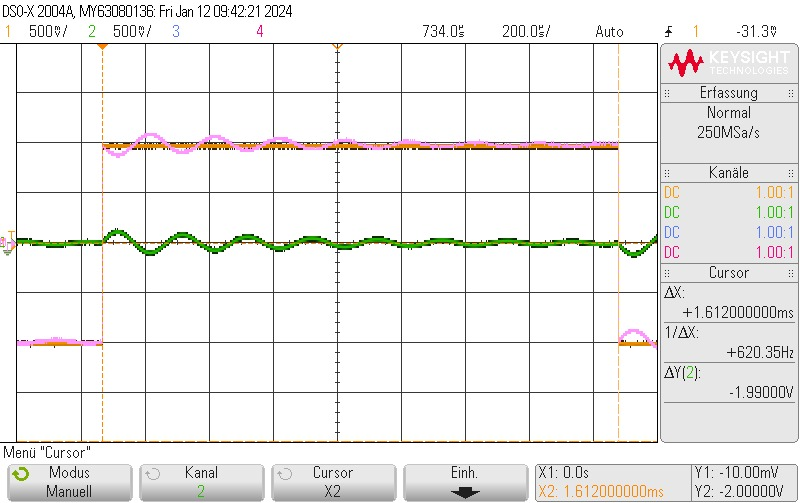
\includegraphics[width=0.6\linewidth]{nudes/Oszi aufgabe 3.jpg}
    \caption{Screenshot des Oszilloskopes mit den Messungen für RLC Parallelschwingkreis. }
    \label{fig:oszi aufgabe 3} 
\end{figure}


\subsection{RLC Serienschwingkreis}
Die Schaltung wird wie in Abbildung \ref{fig:a4b} aufgebaut. 
Mit $L = (10m \pm 10 \mu)H$ und $C = (100 \pm 1)nF$. Der Widerstand $R2A$ wird mit dem Multimeter gemessen und hat den Wert von $R2A = (22 \pm 1) \Omega$. 
Der Channel 1 des Oszilloskopes entspricht der Eingangsspannung $U_{CH1} = U_E$. 
Der Channel 3 des Oszilloskopes entspricht der Spannung am Widerstand $R2A$: $U_{CH3} = U_R$. 
Um die Spannung am Kondensator $U_C$ und der Spule $U_L$ zu bestimmen wird die ''Math'' Funktion des Oszilloskopes verwendet. Dabei ist $U_C = U_{CH1} - U_{CH2}$ und $U_L = U_{CH2} - U_{CH3}$. 
Desweiteren wird auch die Phasenverschiebung $\varphi_{UI}$ zwischen $U_E$ und $U_R$ durch die ''Measure'' Funktion des Oszilloskopes bestimmt. 

\begin{table}[H]
    \centering
    \caption{Messwerte der oben genannten Größen. }
    \label{tab:mess4}
    \begin{tabular}{| l | l | l | l | l | l | l |}
        \hline
        $f$ $\pm$ 0.5 / Hz   & $U_E$ $\pm$ 0.01 / V   & $U_{CH2}$ $\pm$ 1 / V & $U_R$ $\pm$ 0.01 / mV  & $\varphi_{EA}$ $\pm$ 1 / deg. & $U_C$ $\pm$ 0.01 / V & $U_L$ $\pm$ 0.01 / V  \\
        \hline
        4000 & 2.05 & 3.22 & 275 & -77 & 5.05 & 3.22 \\
        4100 & 2.03 & 3.62 & 300 & -75 & 5.34 & 3.61 \\
        4200 & 2.03 & 4.06 & 330 & -73 & 5.72 & 4.04 \\
        4300 & 2.03 & 4.54 & 360 & -72 & 6.12 & 4.52 \\
        4400 & 2.04 & 5.07 & 392 & -68 & 6.56 & 5.04 \\
        4500 & 2.04 & 5.67 & 426 & -64 & 6.98 & 5.64 \\
        4600 & 2.05 & 6.27 & 460 & -60 & 7.41 & 6.24 \\
        4700 & 2.04 & 6.87 & 498 & -51 & 7.77 & 6.83 \\
        4800 & 2.04 & 7.36 & 523 & -40 & 8.01 & 7.35 \\
        4900 & 2.05 & 7.76 & 539 & -20 & 8.07 & 7.70 \\
        5000 & 2.05 & 8.10 & 534 &   7 & 7.95 & 8.02 \\
        5100 & 2.04 & 8.10 & 531 &  27 & 7.63 & 8.08 \\
        5200 & 2.05 & 8.04 & 515 &  42 & 7.27 & 7.95 \\
        5300 & 2.05 & 7.66 & 482 &  53 & 6.77 & 7.65 \\
        5400 & 2.05 & 7.43 & 458 &  60 & 6.25 & 7.32 \\
        5500 & 2.05 & 7.07 & 426 &  64 & 5.77 & 7.00 \\
        5600 & 2.05 & 6.73 & 402 &  69 & 5.30 & 6.67 \\
        5700 & 2.05 & 6.44 & 370 &  70 & 4.89 & 6.34 \\
        5800 & 2.05 & 6.05 & 350 &  72 & 4.50 & 6.02 \\
        5900 & 2.05 & 5.81 & 330 &  74 & 4.14 & 5.72 \\
        \hline
    \end{tabular}
\end{table}

\section{Auswertung und Unsicherheitsanalyse} %Nicht nur zahlen angeben ------------------------------

In der Auswertung werden zur erhöhten Genauigkeit durchgehend ungerundete Werte bis zu den Endergebnissen verwendet und nur zur Darstellung gerundet. \\
Zur Berechnung der Unsicherheiten wird die Größtunsicherheitsmethode verwendet.
\\
\\
Anmerkung. Da die Unsicherheiten teilweise sehr klein ausfallen kann es sein, dass diese in den Diagrammen nicht sichtbar sind. 
\\
\\
\subsection{Hochpass}
Aus den Messdaten der Tabelle \ref{tab:mess1} wird das Bodediagramm erstellt. 
Die Werte der Tabelle werden in QTI-Plot exportiert. 
Der Amplitudengang berechnet sich aus der Differenz der Ausgangsspannung $U_A$ zur Eingangsspannung $U_E$ ($U_A$/$U_E$) und besitzt somit keine Einheit. 
Beim Plot des Bodediagrammes des Amplitudenganges ist zu beachten, die Achsen logarithmisch darzustellen. 
Für das Bodediagramm des Phasengangs wird jedoch nur die x-Achse logarithmisch skaliert. Die y-Achse bleibt linear skaliert. 

\begin{figure}[H]
    \centering
    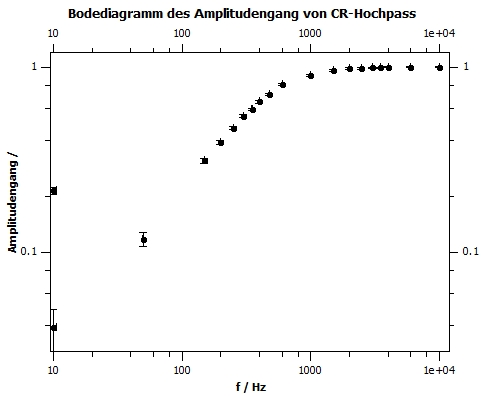
\includegraphics[width=0.6\linewidth]{nudes/Plot a1 amp.jpg}
    \caption{Amplitudengang (y-Achse, log) in Abhängigkeit der Frequenz $f$ (x-Achse, log) eines CR-Hochpasses. }
    \label{fig:plot a1 amp} 
\end{figure}

\begin{figure}[H]
    \centering
    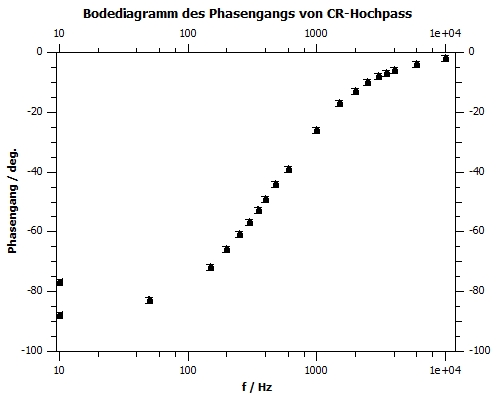
\includegraphics[width=0.6\linewidth]{nudes/Plot a1 ph.jpg}
    \caption{Phasengang (y-Achse, lin) in Abhängigkeit der Frequenz $f$ (x-Achse, log) eines CR-Hochpasses. }
    \label{fig:plot a1 ph} 
\end{figure}

\subsection{Tiefpass}
Die Messdaten der Tabelle \ref{tab:mess2} werden in QTI-Plot exportiert. 
Wie zuvor ist auf die korrekte skalierung der Achsen zu achten. 

\begin{figure}[H]
    \centering
    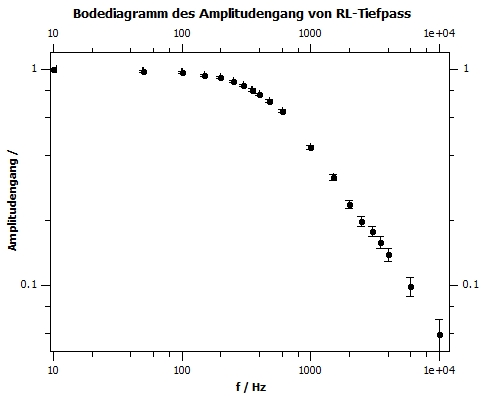
\includegraphics[width=0.6\linewidth]{nudes/Plot a2 amp.jpg}
    \caption{Amplitudengang (y-Achse, log) in Abhängigkeit der Frequenz $f$ (x-Achse, log) eines RL-Tiefpasses. }
    \label{fig:plot a2 amp} 
\end{figure}

\begin{figure}[H]
    \centering
    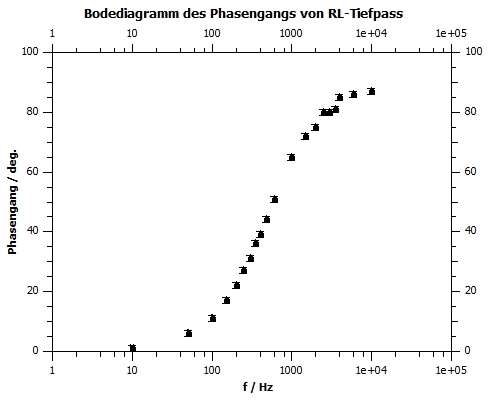
\includegraphics[width=0.6\linewidth]{nudes/Plot a2 ph.jpg}
    \caption{Phasengang (y-Achse, lin) in Abhängigkeit der Frequenz $f$ (x-Achse, log) eines RL-Tiefpasses. }
    \label{fig:plot a2 ph} 
\end{figure}

\subsection{RLC Parallelschwingkreis}
Lädt man die CSV Datei in QTI-Plot, so erhält man alle Daten der aufgenommenen Funktion. 
Gesucht ist dabei der Strom in Abhängigkeit der Zeit. Dieser lässt sich über das Ohm'sche Gesetz berechnen indem man die Spannung $U_R$ durch den Widerstand $R_3$ dividiert. 
Hier ist wieder darauf zu achten, die Achsen linear zu skalieren. 

\begin{figure}[H]
    \centering
    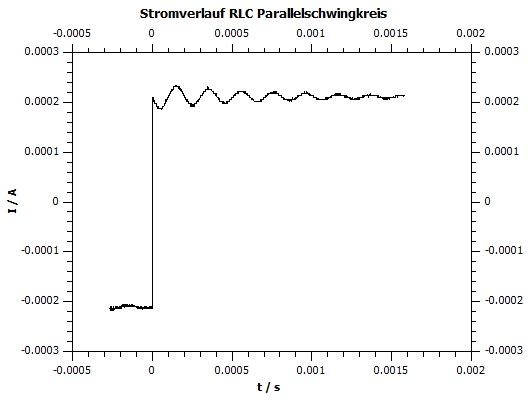
\includegraphics[width=0.6\linewidth]{nudes/Plot a3.jpg}
    \caption{Strom $I$ (y-Achse, lin) in Abhängigkeit der Zeit $t$ (x-Achse, lin) eines RLC-Parallelschwingkreis. }
    \label{fig:plot a3} 
\end{figure}

\noindent
Mithilfe der Zoom- und Datareader Funktion in QTI-Plot lässt sich die Periodendauer bestimmen. Diese beträgt $\Delta t = (0.00019 \pm 0.00001) s$. 
Mithilfe dieser lässt sich die Grenzfrequenz $\omega_0 = (33070 \pm 0.5)$ (Unsicherheit implizit bestimmt) bestimmen. 
Mithilfe der Formeln \ref{eq:wgo} und \ref{eq:wgu} lassen sich die Obere- und Untere Grenzfrequenz bestimmen. 
Diese haben die Werte $\omega_{go} = (471972 \pm 4647) Hz$ und $\omega_{go} = (2317.4 \pm 23) Hz$
Setzt man diese Werte in die Bandbreite $B$ (Formel \ref{eq:Bandbreite}) ein so erhält man den Wert von $B = (469600 \pm 4647)$. 
\\
\\
Da es sich um einen Parallelschwingkreis handelt, benötigt man den Kehrwert der Formel \ref{eq:Güte}. 
Man erhält für die Güte $Q = (14.20 \pm 0.15)$ und parallel dazu die Dämpfung $d = (0.0705 \pm 0.0007)$. 

\subsection{RLC Seriellschwingkreis}
Die Messdaten der Tabelle \ref{tab:mess4} werden in QTI-Plot exportiert. 
Dort lassen sich die Amplitudengänge der einzelnen Spannungen darstellen. 
Es werden der Amplitudengang des Widerstandes $U_R/U_E$, des Kondensators $U_C/U_E$ und der Spule $U_L/U_E$ dargestellt. 
Es ist auf die richtige Skalierung der Achsen zu achten. 
\begin{figure}[H]
    \centering
    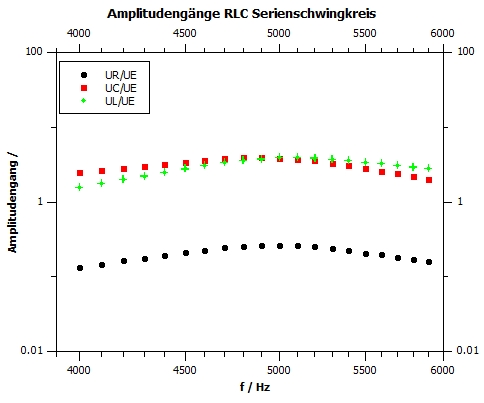
\includegraphics[width=0.6\linewidth]{nudes/Plot a4 amp.jpg}
    \caption{Amplitudengänge (y-Achse, log) in Abhängigkeit der Frequenz $f$ (x-Achse, log) eines RLC-Seriellschwingkreis. }
    \label{fig:plot a4 amp} 
\end{figure}

\noindent
Um die Impendanz $X$ zu berechnen, dividiert man die einzelnen Spannungen durch den zuvor berechneten Strom $I$. 
Für die Gesamtimpendanz $X_ges$ addiet man die Einzelimpendanzen sowie den Widerstand $R$. 

\begin{figure}[H]
    \centering
    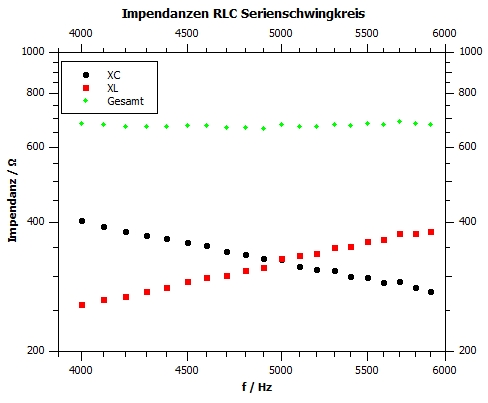
\includegraphics[width=0.6\linewidth]{nudes/Plot a4 imp.jpg}
    \caption{Impendanzen $X$ (y-Achse, log) in Abhängigkeit der Frequenz $f$ (x-Achse, log) eines RLC-Seriellschwingkreis. }
    \label{fig:plot a4 imp} 
\end{figure}

\noindent
Aus der Tabelle \ref{tab:mess4} lässt sich noch der Phasengang in Abhängigkeit der Frequenz darstellen. 
Hier verläuft der Phasengang zwischen Spannung $U$ und Strom $I$. 

\begin{figure}[H]
    \centering
    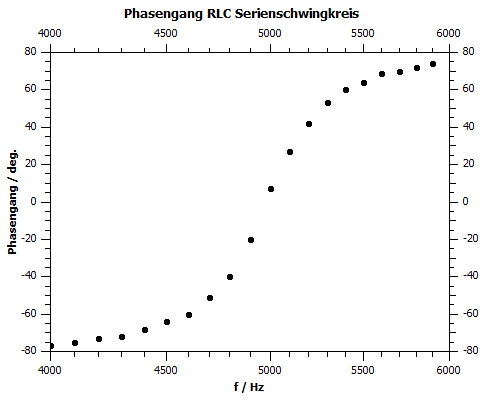
\includegraphics[width=0.6\linewidth]{nudes/Plot a4 ph.jpg}
    \caption{Phasengang (y-Achse, lin) in Abhängigkeit der Frequenz $f$ (x-Achse, log) eines RLC-Seriellschwingkreis. }
    \label{fig:plot a4 ph} 
\end{figure}

\section{Diskussion} %diskussion der Unsicherheiten und Ergebnisse und evtl. verlgeich mit Literatur ------------------------------
\subsection{Hochpass}
Vergleicht man die Bodediagramme mit dem theoretisch berechneten Verlauf, so lässt sich erkennen, dass es einen ähnlichen Verlauf zeigt. 
Es lässt sich daher auf eine fehlerfreie Durchführung schließen. 

\begin{figure}[H]
    \centering
    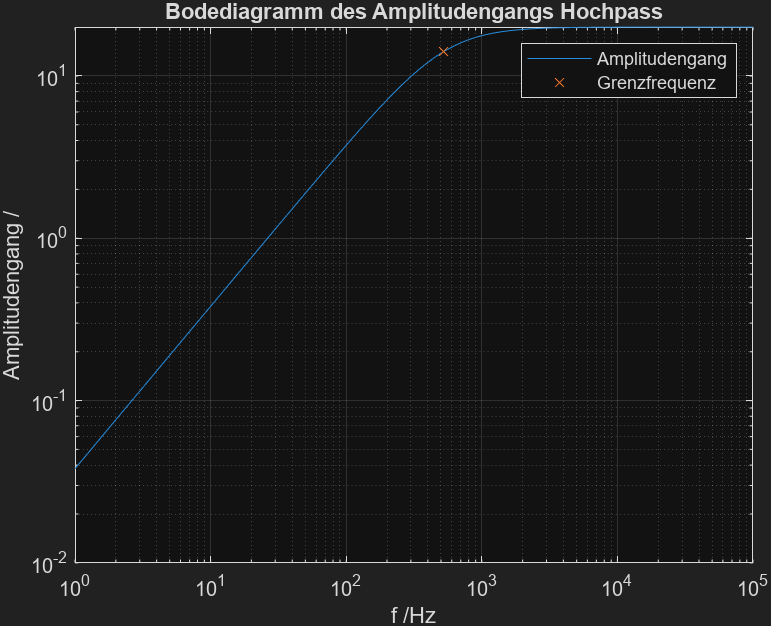
\includegraphics[width=0.6\linewidth]{Matlab/1 amp.png}
    \caption{Theoretisch berechneter Wert des Amplitudenganges für den CR Hochpass.}
    \label{fig:disk 1 amp} 
\end{figure}

\begin{figure}[H]
    \centering
    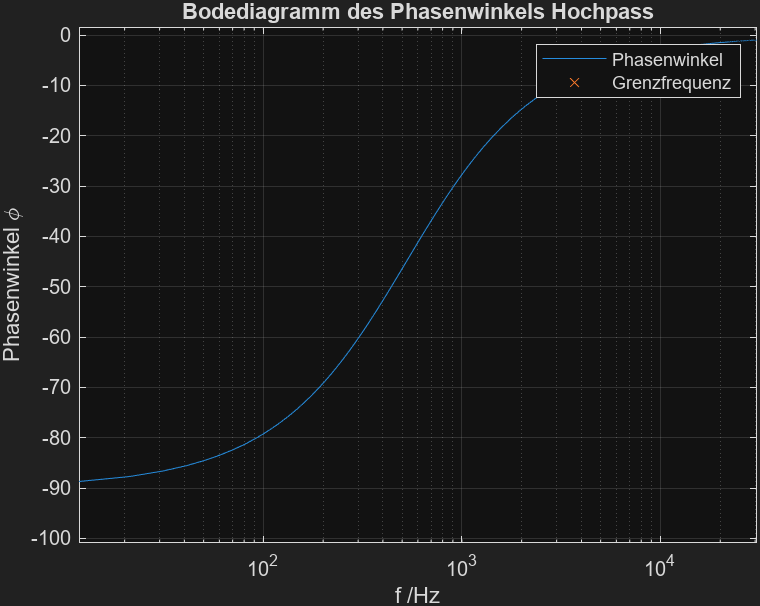
\includegraphics[width=0.6\linewidth]{Matlab/1 ph.png}
    \caption{Theoretisch berechneter Wert des Phasengangs für den CR Hochpass.}
    \label{fig:disk 1 ph} 
\end{figure}

\subsection{Tiefpass}
Vergleicht man die Bodediagramme mit dem theoretisch berechneten Verlauf, so lässt sich erkennen, dass es einen ähnlichen Verlauf zeigt. 
Es lässt sich daher auf eine fehlerfreie Durchführung schließen. 

\begin{figure}[H]
    \centering
    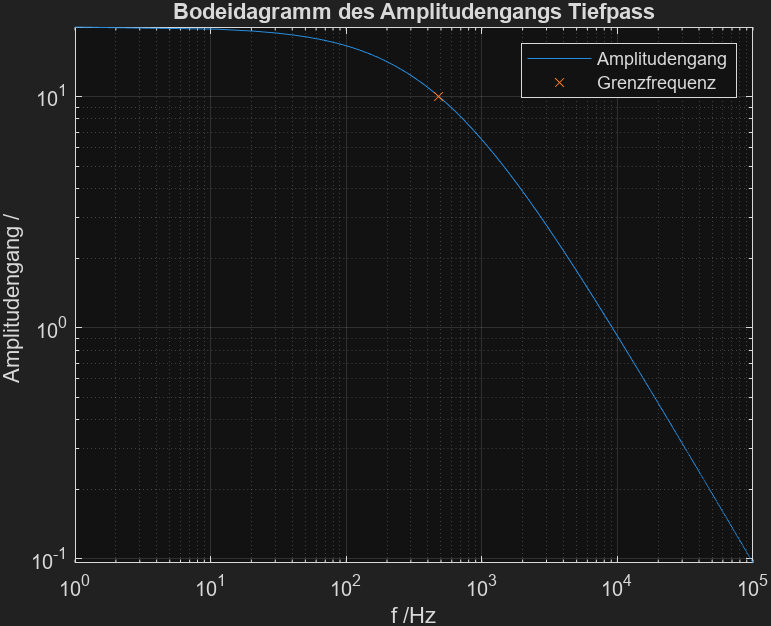
\includegraphics[width=0.6\linewidth]{Matlab/2 amp.png}
    \caption{Theoretisch berechneter Wert des Amplitudenganges für den RC Tiefpass.}
    \label{fig:disk 2 amp} 
\end{figure}

\begin{figure}[H]
    \centering
    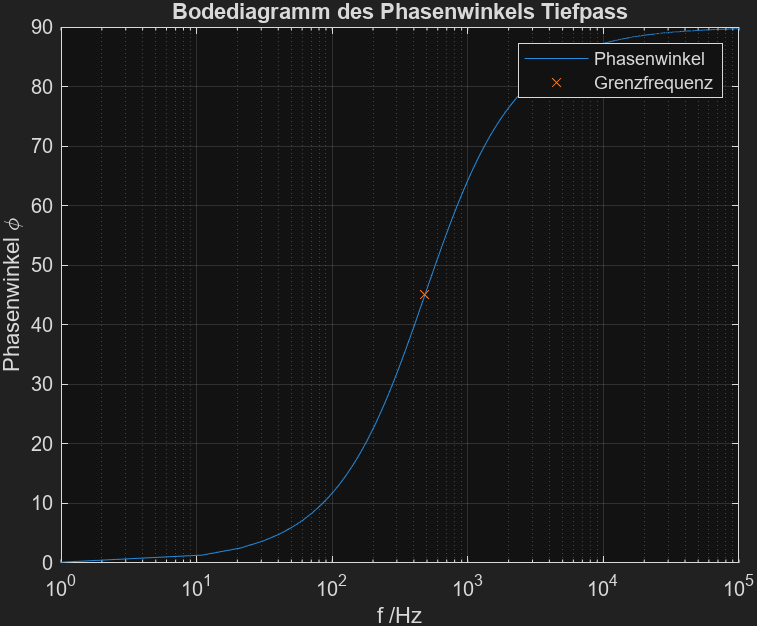
\includegraphics[width=0.6\linewidth]{Matlab/2 ph.png}
    \caption{Theoretisch berechneter Wert des Phasengangs für den RC Tiefpass.}
    \label{fig:disk 2 ph} 
\end{figure}

\subsection{RLC Parallelschwingkreis}
Durch die Gütegleichung eines Serienschwingkreises

\begin{equation}
    \label{eq:Gütegleichung}
    \centerline{$Q_g = \frac{\sqrt{\frac{L}{C}}}{R}$ \\ $\Delta Q_g = \vert \frac{\partial Q_g}{\partial L} * \Delta L \vert + \vert \frac{\partial Q_g}{\partial C} * \Delta C \vert + \vert \frac{\partial q_g}{\partial R} * \Delta R \vert$}
\end{equation}

\noindent 
und dessen Kehrwert lässt sich durch die bekannten Bauteile $R3$, $L$ und $C$ die Güte $Q_g = (14.9 \pm 0.6) $ berechnen. 
Da der berechnete Wert dem der Gütegleichung mit Unsicherheit dem in der Auswertung berechneten Wert von $Q = (14.20 \pm 0.15) $ überschneidet, lässt sich auch hier auf eine fehlerfreie Durchführung schließen. 

\subsection{RLC Seriellschwingkreis}
Vergleicht man den wert der Impendanzen mit dem theoretisch berechneten Verläufen, so lässt sich erkennen, dass es einen ähnlichen Verlauf zeigt. 
Es lässt sich daher auf eine fehlerfreie Durchführung schließen. 

\begin{figure}[H]
    \centering
    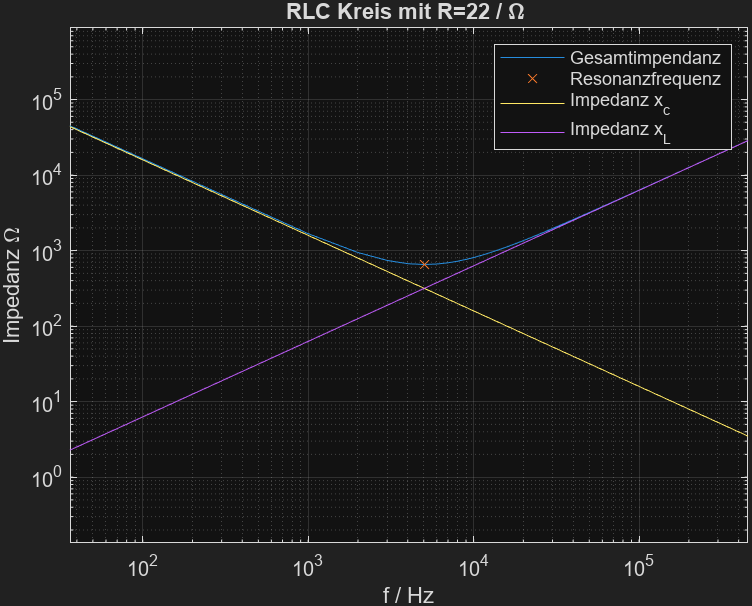
\includegraphics[width=0.6\linewidth]{Matlab/4.png}
    \caption{Theoretisch berechneter Wert der Impendanzen.}
    \label{fig:disk 4} 
\end{figure}

\section{Zusammenfassung} %klare, übersichtliche vollständige beantwortung der Aufgabenstellung ------------------------------
Hier nocheinmal alle Werte zusammengefasst. 

\subsection{Hochpass}
\begin{figure}[H]
    \centering
    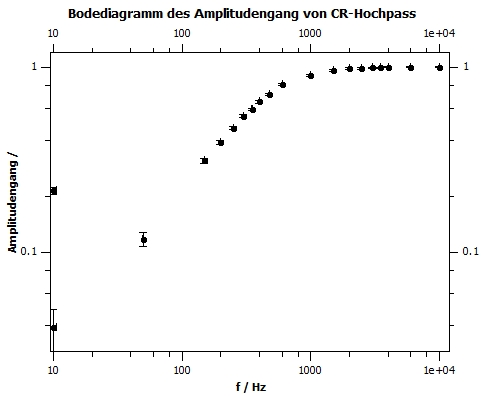
\includegraphics[width=0.6\linewidth]{nudes/Plot a1 amp.jpg}
    \caption{Amplitudengang (y-Achse, log) in Abhängigkeit der Frequenz $f$ (x-Achse, log) eines CR-Hochpasses. }
    \label{fig:zus a1 amp} 
\end{figure}

\begin{figure}[H]
    \centering
    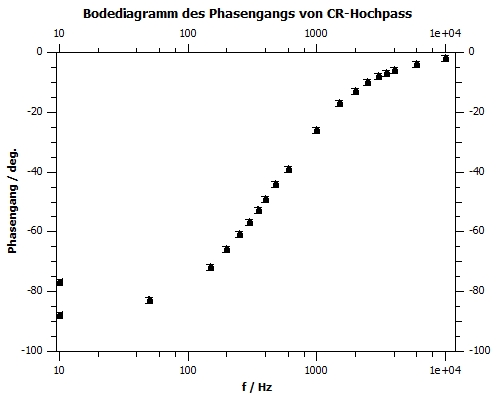
\includegraphics[width=0.6\linewidth]{nudes/Plot a1 ph.jpg}
    \caption{Phasengang (y-Achse, lin) in Abhängigkeit der Frequenz $f$ (x-Achse, log) eines CR-Hochpasses. }
    \label{fig:zus a1 ph} 
\end{figure}

\subsection{Tiefpass}
\begin{figure}[H]
    \centering
    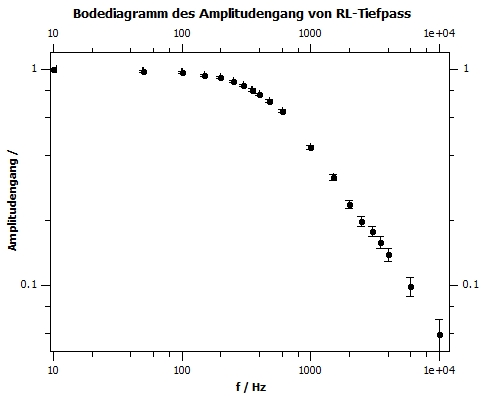
\includegraphics[width=0.6\linewidth]{nudes/Plot a2 amp.jpg}
    \caption{Amplitudengang (y-Achse, log) in Abhängigkeit der Frequenz $f$ (x-Achse, log) eines RL-Tiefpasses. }
    \label{fig:zus a2 amp} 
\end{figure}

\begin{figure}[H]
    \centering
    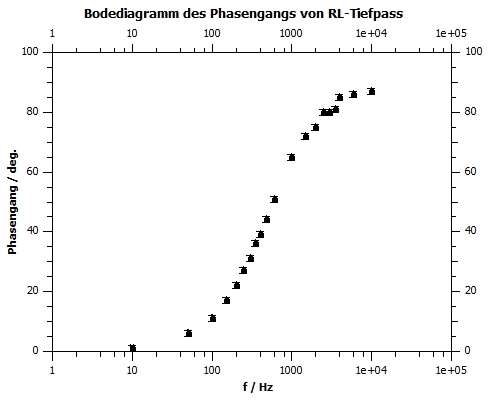
\includegraphics[width=0.6\linewidth]{nudes/Plot a2 ph.jpg}
    \caption{Phasengang (y-Achse, lin) in Abhängigkeit der Frequenz $f$ (x-Achse, log) eines RL-Tiefpasses. }
    \label{fig:zus a2 ph} 
\end{figure}

\subsection{RLC Parallelschwingkreis}
\begin{figure}[H]
    \centering
    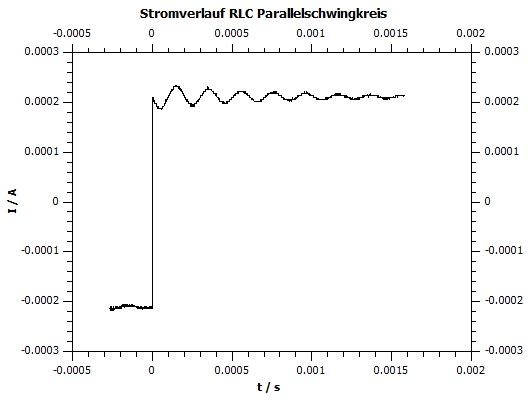
\includegraphics[width=0.6\linewidth]{nudes/Plot a3.jpg}
    \caption{Strom $I$ (y-Achse, lin) in Abhängigkeit der Zeit $t$ (x-Achse, lin) eines RLC-Parallelschwingkreis. }
    \label{fig:zus a3} 
\end{figure}

\noindent
$Q = (14.20 \pm 0.15)$

\subsection{RLC Serienschwingkreis}

\begin{figure}[H]
    \centering
    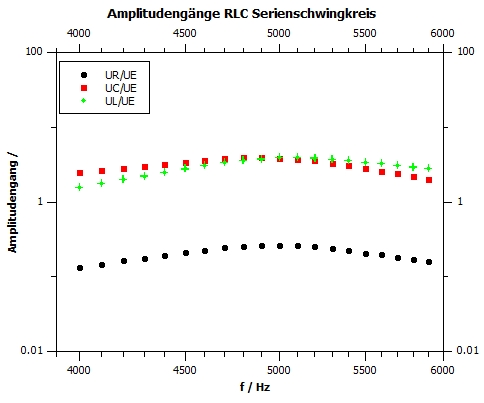
\includegraphics[width=0.6\linewidth]{nudes/Plot a4 amp.jpg}
    \caption{Amplitudengänge (y-Achse, log) in Abhängigkeit der Frequenz $f$ (x-Achse, log) eines RLC-Seriellschwingkreis. }
    \label{fig:zus a4 amp} 
\end{figure}

\begin{figure}[H]
    \centering
    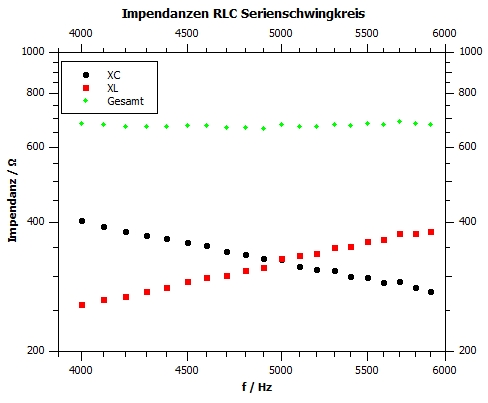
\includegraphics[width=0.6\linewidth]{nudes/Plot a4 imp.jpg}
    \caption{Impendanzen $X$ (y-Achse, log) in Abhängigkeit der Frequenz $f$ (x-Achse, log) eines RLC-Seriellschwingkreis. }
    \label{fig:zus a4 imp} 
\end{figure}

\begin{figure}[H]
    \centering
    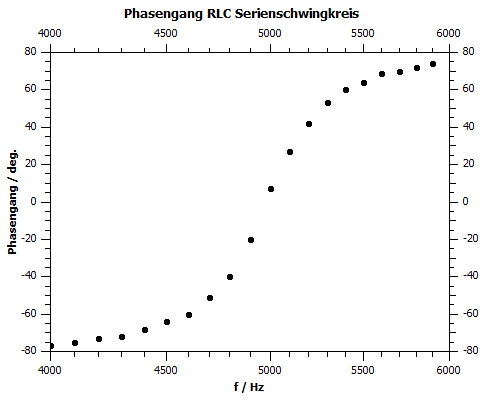
\includegraphics[width=0.6\linewidth]{nudes/Plot a4 ph.jpg}
    \caption{Phasengang (y-Achse, lin) in Abhängigkeit der Frequenz $f$ (x-Achse, log) eines RLC-Seriellschwingkreis. }
    \label{fig:zus a4 ph} 
\end{figure}

\printbibliography[heading=bibintoc]
\end{document}
